\section{Diseño} \label{sec:7_diseno}
En esta sección se describe la especificación del diseño del sistema, proporcionando 
una visión global de la arquitectura. Se describen los principales
componentes y sus interacciones, con el fin de facilitar la comprensión de la estructura 
interna y las decisiones de diseño adoptadas.

\subsection{Visión general} \label{subsec:7_1_visión_general}
El sistema desarrollado tiene dos objetivos. Por un lado, proporcionar una interfaz 
gráfica sencilla, que permita la carga de imágenes en formato crudo y la aplicación de
filtros y operaciones de procesamiento. Este proceso tiene como propósito la definición 
interactiva de \textit{pipelines} de procesado de imágenes. Estos \textit{pipelines} 
deben poder ser exportados a un formato estándar. 

Por otra parte, el sistema debe incorporar un módulo de \textit{benchmarking}
que permita analizar el rendimiento computacional de los \textit{pipelines} definidos. 
Este módulo debe permitir la importación de los \textit{pipelines} creados desde la 
interfaz gráfica y su ejecución en diferentes condiciones experimentales.

\subsubsection{Principios de diseño} \label{subsubsec:7_1_1_principios_de_diseno}
\noindent{Para lograr los objetivos planteados, se han seguido los siguientes principios de diseño:}

\begin{itemize}[noitemsep]
    \item \textbf{Separación de responsabilidades.} Distinción clara entre componentes
    encargados de funciones específicas, minimizando las dependencias entre ellos.
    \item \textbf{Modularidad.} Funcionalidades encapsuladas en módulos bien 
    definidos, permitiendo ampliar partes del sistema sin afectar al conjunto.
    \item \textbf{Simplicidad y claridad estructural.} Se evita introducir complejidad innecesaria, 
    manteniendo flujos de trabajo y relaciones entre módulos fácilmente identificables.
\end{itemize}

\subsubsection{Flujo de ejecución} \label{subsubsec:7_1_2_flujo_de_ejecucion}
De forma esquemática, el flujo de ejecución del sistema se divide en dos grandes bloques funcionales:
la interfaz gráfica y el módulo de \textit{benchmarking}. Se muestra
en la Figura \ref{fig:32_flujo_ejecucion_sistema}.

\begin{figure}[h!]
    \centering
    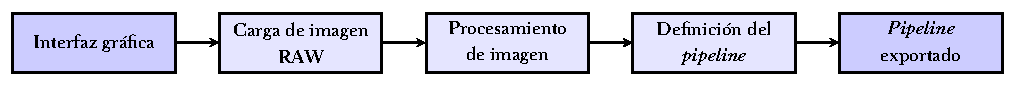
\includegraphics[width=\textwidth]{tikz_figures/system_execution_flow/system_execution_flow_1.pdf}
    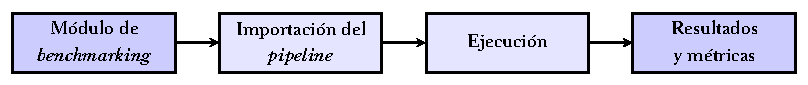
\includegraphics[width=0.8\textwidth]{tikz_figures/system_execution_flow/system_execution_flow_2.pdf}
    \caption{Flujo general de ejecución del sistema}
    \label{fig:32_flujo_ejecucion_sistema}
\end{figure}

\newpage

\subsection{Arquitectura} \label{subsec:7_2_arquitectura}
Se presenta a continuación la arquitectura del sistema desarrollado. Dicha arquitectura
se ha planteado y diseñado siguiendo los objetivos y principios mencionados anteriormente.
Finalmente, se muestra un diagrama de clases simplificado que complementa la vista 
arquitectónica general.

\subsubsection{Enfoque arquitectónico} \label{subsubsec:7_2_1_enfoque_arquitectonico}
El sistema desarrollado sigue un enfoque de arquitectura en capas, combinando el patrón 
MVC \cite{mvc_pattern} con un modelo de ejecución basado en \textit{pipelines} de 
procesamiento.

El patrón MVC facilita el desarrollo de la aplicación interactiva, manteniendo desacoplada la 
interfaz gráfica de la lógica de negocio y de las estructuras de datos y entidades principales.
De este modo, las acciones del usuario se traducen en eventos gestionados por un controlador, 
que coordina la actualización del estado de la aplicación y la representación visual.

Por otra parte, el modelo de ejecución basado en \textit{pipelines} permite definir secuencias
de operaciones de procesamiento de imágenes, favoreciendo su reutilización y exportación. 
Esto facilita la integración con el módulo de \textit{benchmarking}.

La \autoref{fig:33_arch_diagram} muestra el diagrama general de arquitectura del sistema, donde se identifican 
los principales componentes y sus interacciones. Cada uno de ellos tiene un rol específico, actuando 
de forma coordinada para cumplir con los objetivos funcionales.

\begin{figure}[h!]
    \centering
    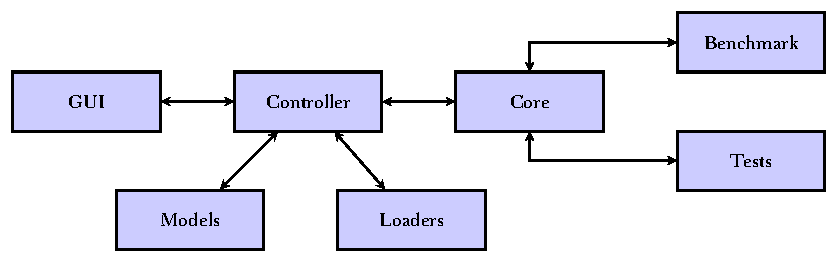
\includegraphics[width=0.8\textwidth]{tikz_figures/architecture/architecture.pdf}
    \caption{Diagrama de arquitectura del sistema}
    \label{fig:33_arch_diagram}
\end{figure}

A partir de esta organización, se logra una arquitectura modular, mantenible y fácilmente extensible,
en la que es posible incorporar nuevas operaciones de procesamiento de imágenes, ampliar el 
soporte de formatos de entrada o introducir nuevas métricas de rendimiento de forma muy sencilla, 
sin afectar al conjunto global del sistema. 

\newpage

\clearpage
\KOMAoptions{paper=landscape,DIV=6}
\newgeometry{top=3.5cm, bottom=2.5cm, left=2.3cm, right=2.3cm}
\setlength{\headheight}{49.60443pt}
\addtolength{\topmargin}{-30.05453pt}
\fancyheadoffset{0pt}

\thispagestyle{fancy}

\subsubsection{Diagrama de clases} \label{subsubsec:7_2_2_diagrama_clases}
Como complemento a la vista arquitectónica anterior, la \autoref{fig:34_class_diagram} muestra una
representación estática simplificada de las clases principales de la aplicación y de sus relaciones más
relevantes. Dichas clases y elementos se describen en detalle en las secciones siguientes.

\begin{figure}[h!]
    \centering
    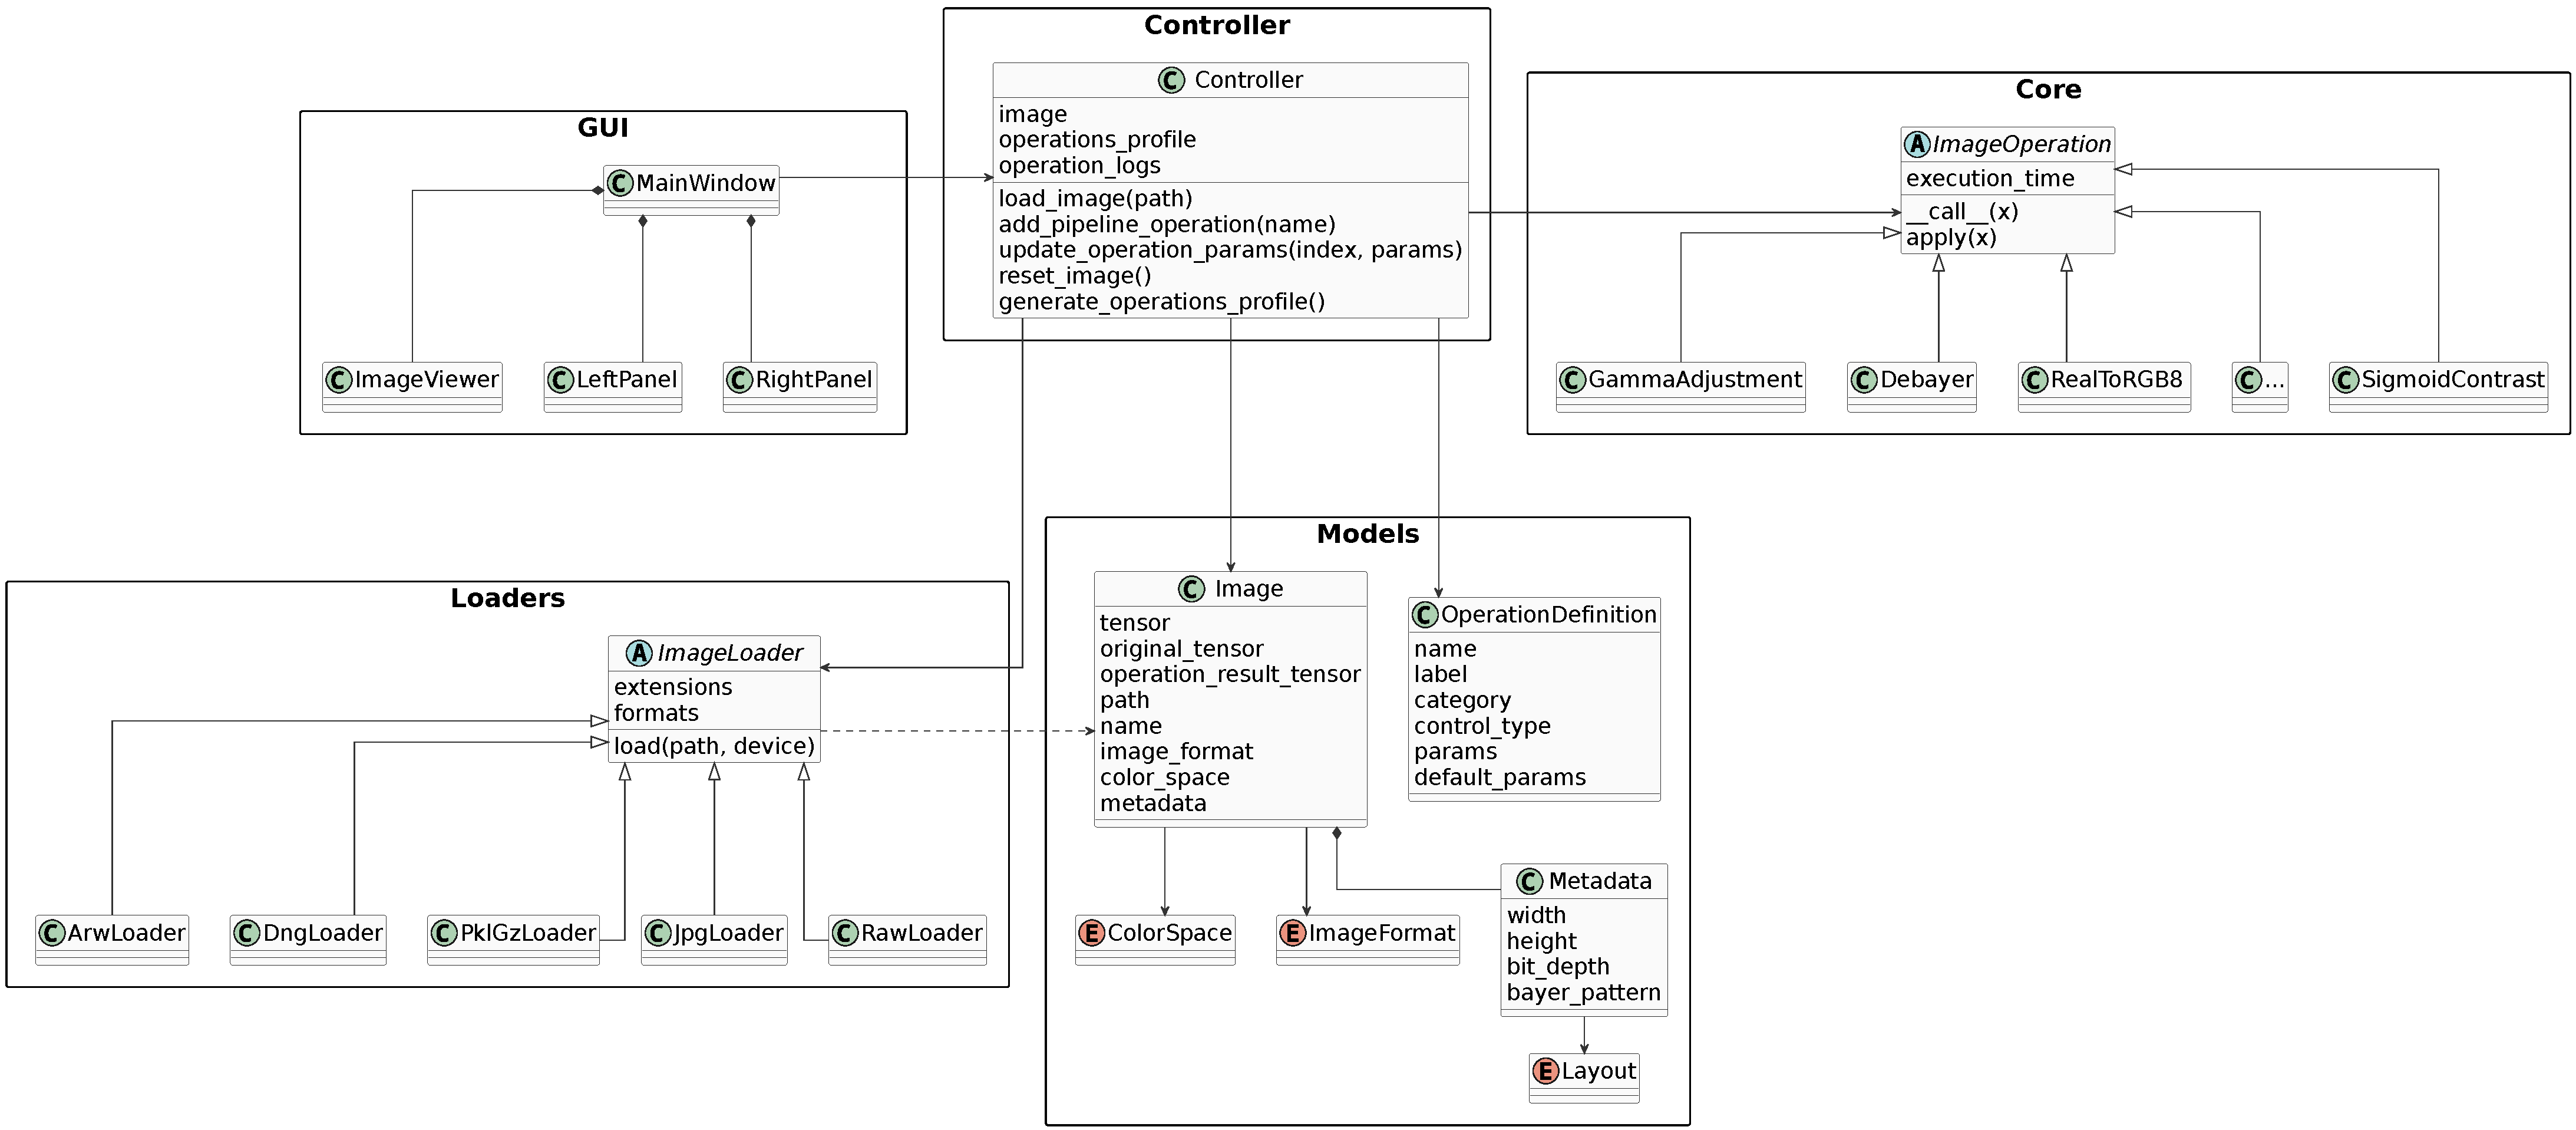
\includegraphics[width=\textwidth]{puml_figures/class_diagram/application_class_diagram.pdf}
    \caption{Diagrama de clases simplificado de la aplicación}
    \label{fig:34_class_diagram}
\end{figure}

\clearpage
\addtolength{\topmargin}{30.05453pt}
\KOMAoptions{paper=portrait,DIV=last}
\restoregeometry
\fancyheadoffset{0pt}


\newpage

\subsection{Componentes} \label{subsubsec:7_3_componentes}
En esta sección, se describen en detalle los componentes principales que conforman el sistema.
Se definen sus funciones, responsabilidades y los criterios de diseño específicos que rigen 
su implementación.

\subsubsection{Models} \label{subsubsec:7_3_1_models}
El componente \textit{Models} define las estructuras de datos del sistema, encapsulando 
la representación de imágenes, operaciones y sus metadatos asociados. Este componente sigue el 
patrón de diseño \textit{Data Transfer Object} (DTO) y utiliza \textit{dataclasses} 
\cite{python_dataclasses} de Python para garantizar inmutabilidad y validación de tipos.
Se organiza en dos niveles:

\begin{itemize}[noitemsep]
    \item \textbf{Modelos}. Clases que representan las entidades centrales del sistema: 
    \textit{Image}, \textit{Metadata}, \textit{OperationDefinition} y \textit{FloatParamSpec}.
    \item \textbf{Enumeraciones}. Tipos enumerados que definen valores válidos para espacios de 
    color, formatos de imagen y patrones Bayer: \textit{ColorSpace}, \textit{ImageFormat} y \textit{Layout},
    respectivamente.
\end{itemize}

\noindent{A continuación, se describen las clases y enumeraciones de mayor relevancia.}

\paragraph{Clase \textit{Image}} \label{par:7_3_1_1_image}
Constituye el modelo central, representando el estado completo de una imagen durante su procesamiento.
Sus atributos principales son:

\begin{itemize}[noitemsep]
    \item \texttt{\textbf{tensor}} $\rightarrow$ Tensor con el estado actual de la imagen.
    \item \texttt{\textbf{original\_tensor}} $\rightarrow$ Tensor inmutable que preserva la imagen original 
    cargada, permitiendo operaciones de restablecimiento.
    \item \texttt{\textbf{operation\_result\_tensor}} $\rightarrow$ Tensor temporal que almacena el resultado 
    de la última operación aplicada, facilitando la previsualización antes de confirmar cambios.
    \item \texttt{\textbf{path}} y \texttt{\textbf{name}} $\rightarrow$ Información de ubicación e identificación del archivo.
    \item \texttt{\textbf{image\_format}} $\rightarrow$ Enumeración que especifica el formato original del archivo.
    \item \texttt{\textbf{metadata}} $\rightarrow$ Objeto \texttt{Metadata} con información técnica de la imagen.
    \item \texttt{\textbf{color\_space}} $\rightarrow$ Espacio de color actual.
\end{itemize}

\newpage

\paragraph{Clase \textit{Metadata}} \label{par:7_3_1_2_metadata}
\noindent{Encapsula los metadatos técnicos asociados a una imagen. Sus atributos incluyen:}

\begin{itemize}[noitemsep]
    \item \texttt{\textbf{width}} y \texttt{\textbf{height}} $\rightarrow$ Dimensiones de la imagen en píxeles.
    \item \texttt{\textbf{bit\_depth}} $\rightarrow$ Profundidad de bits.
    \item \texttt{\textbf{bayer\_pattern}} $\rightarrow$ Patrón del filtro de color Bayer, utilizado 
    en la etapa de demosaicing.
\end{itemize}

\paragraph{Clase \textit{OperationDefinition}} \label{par:7_3_1_3_operation_definition}
Define la especificación completa de una operación de procesamiento de imagen. Actúa como plantilla para 
todas las operaciones disponibles. Utilizada para encapsular datos y parámetros necesarios para la 
ejecución de operaciones desde la interfaz de usuario. Sus atributos principales son:

\begin{itemize}[noitemsep]
    \item \texttt{\textbf{name}} $\rightarrow$ Identificador único de la operación.
    \item \texttt{\textbf{label}} $\rightarrow$ Etiqueta descriptiva para la interfaz de usuario.
    \item \texttt{\textbf{category}} $\rightarrow$ Categoría de agrupación (``Filters'', ``Color'', 
    ``Normalization'', ``Geometry'', ``Format'', ``Bayer'').
    \item \texttt{\textbf{control\_type}} $\rightarrow$ Tipo de control GUI asociado (``filter'', ``no\_param'', 
    ``debayer'', ``flip'', etc.).
    \item \texttt{\textbf{params}} $\rightarrow$ Lista opcional de especificaciones de parámetros 
    (\texttt{FloatParamSpec}).
    \item \texttt{\textbf{default\_params}} $\rightarrow$ Diccionario con valores por defecto de los parámetros.
\end{itemize}

\paragraph{Enumeraciones} \label{par:7_3_1_4_enumeraciones}
Proporcionan validación de tipos y documentación explícita de valores permitidos. Se definen las 
siguientes:

\begin{itemize}[noitemsep]
    \item \texttt{\textbf{ColorSpace}} $\rightarrow$ RGB, HSV y Grayscale.
    \item \texttt{\textbf{ImageFormat}} $\rightarrow$ RAW, ARW, DNG, PKL\_GZ y JPG.
    \item \texttt{\textbf{Layout}} $\rightarrow$ Patrones Bayer (RGGB, GRBG, GBRG, BGGR), donde cada valor 
    representa los índices de color (R=0, G=1, B=2) en un bloque 2×2.
\end{itemize}

\newpage

\subsubsection{Loaders} \label{subsubsec:7_3_2_loaders}
El componente \textit{Loaders} implementa un sistema extensible de carga de imágenes en múltiples 
formatos. Utiliza un patrón de diseño basado en una clase base abstracta \cite{python_abc} que define la interfaz 
común para todos los \textit{loaders}. Esto permite añadir soporte para nuevos formatos de imagen 
sin modificar el código existente. Cada \textit{loader} concreto hereda de esta clase base e implementa la lógica
específica para leer y convertir archivos de un formato particular en objetos \textit{Image}. 
El conjunto de todos los \textit{loaders} disponibles se gestiona mediante un módulo de orquestación 
que contiene un registro dinámico. 

\paragraph{Clase base \textit{ImageLoader}} \label{par:7_3_2_1_image_loader}
\noindent{Define la interfaz común para todos los \textit{loaders} de imágenes:}

\begin{itemize}[noitemsep]
    \item \texttt{\textbf{extensions}} $\rightarrow$ Propiedad que retorna una secuencia de extensiones soportadas 
    en formato de cadena de texto.
    \item \texttt{\textbf{formats}} $\rightarrow$ Propiedad que retorna los valores \texttt{ImageFormat} 
    correspondientes.
    \item \texttt{\textbf{load(path, device)}} $\rightarrow$ Método abstracto que carga una imagen desde la ruta 
    especificada y la coloca en el dispositivo PyTorch indicado, retornando un objeto 
    \texttt{Image} inicializado.
\end{itemize}

\paragraph{Loaders implementados} \label{par:7_3_2_2_loaders}
Se implementan los siguientes \textit{loaders} concretos, para dar soporte a diferentes formatos de imagen cruda: \footnotemark

\begin{itemize}[noitemsep]
    \item \texttt{\textbf{RawLoader}} $\rightarrow$ Soporta archivos con extensión \texttt{.raw}.
    \item \texttt{\textbf{ArwLoader}} $\rightarrow$ Soporta archivos con extensión \texttt{.arw} (Sony).
    \item \texttt{\textbf{DngLoader}} $\rightarrow$ Soporta archivos con extensión \texttt{.dng} (Adobe, Apple).
    \item \texttt{\textbf{PklGzLoader}} $\rightarrow$ Soporta archivos con extensión \texttt{.pkl.gz} 
    (formato personalizado).
\end{itemize}

Con el fin de facilitar el desarrollo y pruebas, también se implementa un \textit{loader} (\texttt{\textbf{JpgLoader}})
que permite cargar imágenes en formato comprimido \texttt{.jpg}. 

\paragraph{Módulo de orquestación} \label{par:7_3_2_3_modulo_orquestacion}
Gestiona la carga automática de imágenes utilizando el \textit{loader} adecuado según la extensión del archivo. 
Proporciona una función \texttt{load\_image(path, device)} que identifica el \textit{loader} correcto
y delega la tarea de carga, retornando un objeto \texttt{Image}. También ofrece una función
\texttt{get\_supported\_formats()} que retorna la lista de todos los formatos de imagen soportados, 
en función de los \textit{loaders} registrados. Este módulo es utilizado por el \textit{Controller} para gestionar 
la carga de imágenes desde la interfaz gráfica.

\footnotetext{Existen numerosos formatos de imagen cruda. Información sobre ellos puede encontrarse en 
el \autoref{sec:appendix_D_raw_formats}.}

\newpage

\subsubsection{Core} \label{subsubsec:7_3_3_core}
Este componente constituye el motor de procesamiento de imágenes. Implementa todas las operaciones de transformación 
siguiendo, de nuevo, un patrón de diseño basado en una clase abstracta. Las operaciones se organizan en varias 
categorías temáticas. Cada operación concreta hereda de la clase base e implementa la lógica específica. 
De esta forma, la implementación de cada operación es completamente autónoma e independiente, además de fácilmente 
\textit{testeable}. También incluye un módulo de utilidades para la gestión de tensores y un sistema de registro 
dinámico de todas las operaciones disponibles.

\paragraph{Clase base \textit{ImageOperation}} \label{par:7_3_3_1_image_operation}
\noindent{Define la interfaz común para todas las operaciones de procesamiento de imágenes:}

\begin{itemize}[noitemsep]
    \item \texttt{\textbf{\_\_call\_\_(x)}} $\rightarrow$ Punto de entrada público que:
    \begin{enumerate}
        \item Valida que la entrada sea un tensor 3D (C,H,W).
        \item Invoca el método abstracto \texttt{apply()}.
        \item Valida que la salida sea un tensor 3D.
        \item Garantiza que el tensor de salida sea contiguo en memoria.
        \item Proporciona validación de tipos de entrada y salida.
    \end{enumerate}
    \item \texttt{\textbf{apply(x)}} $\rightarrow$ Método abstracto que implementa la lógica específica 
    de cada operación.
\end{itemize}

Además, con fines de análisis, la clase base incluye un parámetro (\texttt{execution\_time}) que 
almacena el tiempo de ejecución de la última llamada a la operación, medido en milisegundos.
Esta medida se muestra en la interfaz gráfica para proporcionar retroalimentación al usuario 
sobre el rendimiento de cada operación aplicada.

\paragraph{Sistema de registro} \label{par:7_3_3_2_sistema_registro}
Utiliza un diccionario global (\texttt{OPERATION\_REGISTRY}) que mapea los nombres de las operaciones
a sus clases concretas. Además, proporciona un decorador (\texttt{@register\_operation}) que registra 
automáticamente cada clase de operación al momento de su definición. Este sistema de registro es 
utilizado gestionado por el \textit{Controller} y por el módulo de \textit{benchmarking} de forma 
completamente independiente y dinámica para la invocación de operaciones.

\newpage

\paragraph{Operaciones implementadas} \label{par:7_3_3_3_operaciones_implementadas}
Se implementan todas las operaciones de procesamiento de imágenes descritas previamente en la 
\autoref{subsec:3_5_fundamentos_procesamiento_digital_imagenes}, organizadas en las siguiente 
categorías:

\begin{itemize}[noitemsep]
    \item \texttt{\textbf{Filters}}. Operaciones de filtrado y mejora de contraste.
    \begin{itemize}[noitemsep]
        \item \texttt{\textbf{BrightnessAdjustment}} $\rightarrow$ Ajuste de brillo mediante multiplicación escalar.
        \item \texttt{\textbf{MeanContrastAdjustment}} $\rightarrow$ Ajuste de contraste mediante media.
        \item \texttt{\textbf{AffineIntensityTransformation}} $\rightarrow$ Transformación afín de intensidad para ajuste de brillo y contraste.
        \item \texttt{\textbf{SigmoidContrast}} $\rightarrow$ Mejora de contraste mediante función sigmoide.
        \item \texttt{\textbf{GaussianFilter}} $\rightarrow$ Filtro de desenfoque gaussiano.
        \item \texttt{\textbf{MedianFilter}} $\rightarrow$ Filtro de mediana para reducción de ruido.
        \item \texttt{\textbf{GammaAdjustment}} $\rightarrow$ Ajuste gamma para corrección tonal.
        \item \texttt{\textbf{HistogramEqualization}} $\rightarrow$ Ecualización de histograma.
        \item \texttt{\textbf{CLAHE}} $\rightarrow$ Ecualización adaptativa de histograma con limitación de contraste.
        \item \texttt{\textbf{UnsharpMask}} $\rightarrow$ Máscara de enfoque para realce de bordes.
        \item \texttt{\textbf{LightCompensation}} $\rightarrow$ Compensación de luz mediante matriz de corrección.
        \item \texttt{\textbf{WhiteBalance}} $\rightarrow$ Balance de blancos para corrección de dominantes de color.
    \end{itemize}
    \vspace{0.15cm}
    \item \texttt{\textbf{Color}}. Operaciones de conversión entre espacios de color.
    \begin{itemize}[noitemsep]
        \item \texttt{\textbf{ColorToGray}} $\rightarrow$ Conversión RGB a escala de grises.
        \item \texttt{\textbf{GrayToColor}} $\rightarrow$ Conversión de escala de grises a RGB.
        \item \texttt{\textbf{RgbToHsv}} $\rightarrow$ Conversión de espacio de color RGB a HSV.
        \item \texttt{\textbf{HsvToRgb}} $\rightarrow$ Conversión de espacio de color HSV a RGB.
    \end{itemize}
    \vspace{0.15cm}
    \item \texttt{\textbf{Geometry}}. Transformaciones geométricas sobre la imagen.
    \begin{itemize}[noitemsep]
        \item \texttt{\textbf{Flip}} $\rightarrow$ Volteo horizontal o vertical.
        \item \texttt{\textbf{Rotate}} $\rightarrow$ Rotación de la imagen.
        \item \texttt{\textbf{Resize}} $\rightarrow$ Redimensionamiento de la imagen.
    \end{itemize}
    \vspace{0.15cm}
    \item \texttt{\textbf{Normalization}}. Normalización de valores de píxeles.
    \begin{itemize}[noitemsep]
        \item \texttt{\textbf{MinMaxNormalization}} $\rightarrow$ Normalización Min-Max estándar.
        \item \texttt{\textbf{MinMaxNormalizationWithParams}} $\rightarrow$ Normalización Min-Max con parámetros de rango personalizados.
        \item \texttt{\textbf{MinMaxPercentileNormalization}} $\rightarrow$ Normalización Min-Max con percentiles.
    \end{itemize}
    \vspace{0.15cm}
    \item \texttt{\textbf{Bayer}}. \textit{Demosaicing} de imágenes RAW con patrón Bayer.
    \begin{itemize}[noitemsep]
        \item \texttt{\textbf{Debayer}} $\rightarrow$ Conversión de imagen Bayer monocanal a RGB. Se implementan 
        diferentes módulos de \textit{demosaicing} que implican distintos compromisos entre calidad y rendimiento:
        \begin{itemize}[noitemsep]
            \item \texttt{\textbf{Debayer2x2}} $\rightarrow$ Interpolación bilineal básica.
            \item \texttt{\textbf{Debayer3x3}} $\rightarrow$ Interpolación con kernel 3x3.
            \item \texttt{\textbf{Debayer5x5}} $\rightarrow$ Interpolación con kernel 5x5.
            \item \texttt{\textbf{DebayerSplit}} $\rightarrow$ Método alternativo basado en separación de canales.
        \end{itemize}
    \end{itemize}
    \vspace{0.15cm}
    \item \texttt{\textbf{Format}}. Conversiones de formato de datos.
    \begin{itemize}[noitemsep]
        \item \texttt{\textbf{RealToRGB8}} $\rightarrow$ Conversión de coma flotante a enteros de 8 bits.
        \item \texttt{\textbf{RGB8ToReal}} $\rightarrow$ Conversión de enteros de 8 bits a coma flotante.
    \end{itemize}
\end{itemize}

\newpage

\subsubsection{Controller} \label{subsubsec:7_3_4_controller}
El \textit{Controller} actúa como el coordinador central del sistema. Su responsabilidad principal es la 
orquestación de la interacción entre la interfaz gráfica, los \textit{loaders} y el motor de 
procesamiento (\textit{Core}). Mantiene el estado de la imagen cargada, gestiona el \textit{pipeline} de operaciones 
y mantiene un registro de eventos. A continuación, se describen en detalle sus principales cometidos.

\paragraph{Gestión de la imagen y su estado} \label{par:7_3_4_1_gestion_imagen_estado}
\noindent{Cuando el usuario carga una imagen a través de la interfaz gráfica, el \textit{Controller}}

\begin{enumerate}[noitemsep]
    \item La guarda como imagen actual.
    \item Controla su estado tras la aplicación de operaciones.
    \item Mantiene una copia de referencia de la imagen original para permitir restablecimientos.
\end{enumerate}

Este flujo garantiza que el usuario pueda experimentar con diferentes operaciones sin perder 
la imagen inicial, pero no permite la ejecución secuencial de múltiples operaciones acumulativas. Tampoco 
permite deshacer operaciones individuales.

\paragraph{Gestión del \textit{pipeline} de operaciones} \label{par:7_3_4_2_gestion_pipeline_operaciones}
Para mitigar las limitaciones anteriores, el \textit{Controller} mantiene una lista ordenada de
operaciones que constituyen el \textit{pipeline} de procesamiento definido por el usuario. 
Cuando el usuario aplica una nueva operación, esta se añade al final de la lista, recalculando 
el resultado para toda la secuencia. Esto permite:

\begin{enumerate}[noitemsep]
    \item Aplicar múltiples operaciones de forma acumulativa.
    \item Modificar, reordenar o eliminar operaciones individuales.
    \item Previsualizar el resultado tras cada cambio en el \textit{pipeline}.
\end{enumerate}

Sin embargo, este planteamiento es computacionalmente costoso para \textit{pipelines} largos 
o imágenes de gran tamaño, ya que cada modificación requiere recalcular desde el inicio.

\newpage

\paragraph{Sistema de \textit{snapshots}} \label{par:7_3_4_3_sistema_snapshots}
Para optimizar el rendimiento, el \textit{Controller} implementa un sistema de \textit{snapshots}. Este sistema
guarda estados intermedios de la imagen tras la aplicación de cierto número de operaciones. De este modo,
cuando se modifica una operación en el \textit{pipeline}, el \textit{Controller} puede restaurar el estado 
más reciente guardado antes de la operación modificada y continuar desde ese punto, en lugar de recalcular 
continuamente desde el inicio. En la \autoref{fig:controller_snapshots} se ilustra este concepto.

\begin{figure}[h]
    \centering
    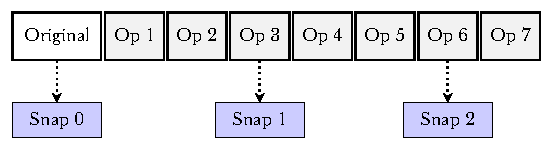
\includegraphics[width=0.6\textwidth]{tikz_figures/snapshot_system/snapshot_system.pdf}
    \caption{Sistema de \textit{snapshots} para optimización del \textit{pipeline} de operaciones}
    \label{fig:controller_snapshots}
\end{figure}

Se observa como, tras aplicar 3 operaciones, se guarda el primer \textit{snapshot} (Snap 1).
Después de aplicar otras 3 operaciones, se guarda el segundo \textit{snapshot} (Snap 2). Si el usuario
modifica la operación 5, el \textit{Controller} puede restaurar el estado desde Snap 1 y continuar desde ahí, 
aplicando las operaciones 5, 6 y 7, en lugar de recalcular desde el estado original.

\paragraph{Actualización de la interfaz} \label{par:7_3_4_4_actualizacion_interfaz}
Por último, el \textit{Controller} es responsable de manejar las actualizaciones de la interfaz gráfica. 
Cuando el usuario realiza una acción (carga de imagen, aplicación de operación, modificación del 
\textit{pipeline}, etc.), el \textit{Controller} procesa la solicitud y notifica a la GUI para que 
refresque la visualización correspondiente. La interfaz siempre representa el estado real del sistema 
y el usuario recibe una respuesta inmediata a sus acciones.

Además, el \textit{Controller} mantiene un registro de todas las acciones realizadas por el usuario
durante una sesión. Dicho registro se muestra en la interfaz en forma de \textit{logger} para proporcionar 
retroalimentación y facilitar el seguimiento de cambios realizados.

\newpage

\subsubsection{GUI} \label{subsubsec:7_3_5_gui}
El componente \textit{GUI} implementa la interfaz gráfica utilizando PyQt6 \cite{pyqt6}. Ocupa varias responsabilidades: 
la presentación de la imagen, el manejo de la interacción del usuario y la visualización de información relevante sobre el procesamiento.
Su diseño sigue una estructura completamente modular, donde cada panel o \textit{widget} tiene una función específica 
bien definida. En la \autoref{fig:35_gui_no_image_loaded_overview} y la \autoref{fig:36_gui_image_loaded_overview}
se muestra una visión general.

\begin{figure}[h!]
    \centering
    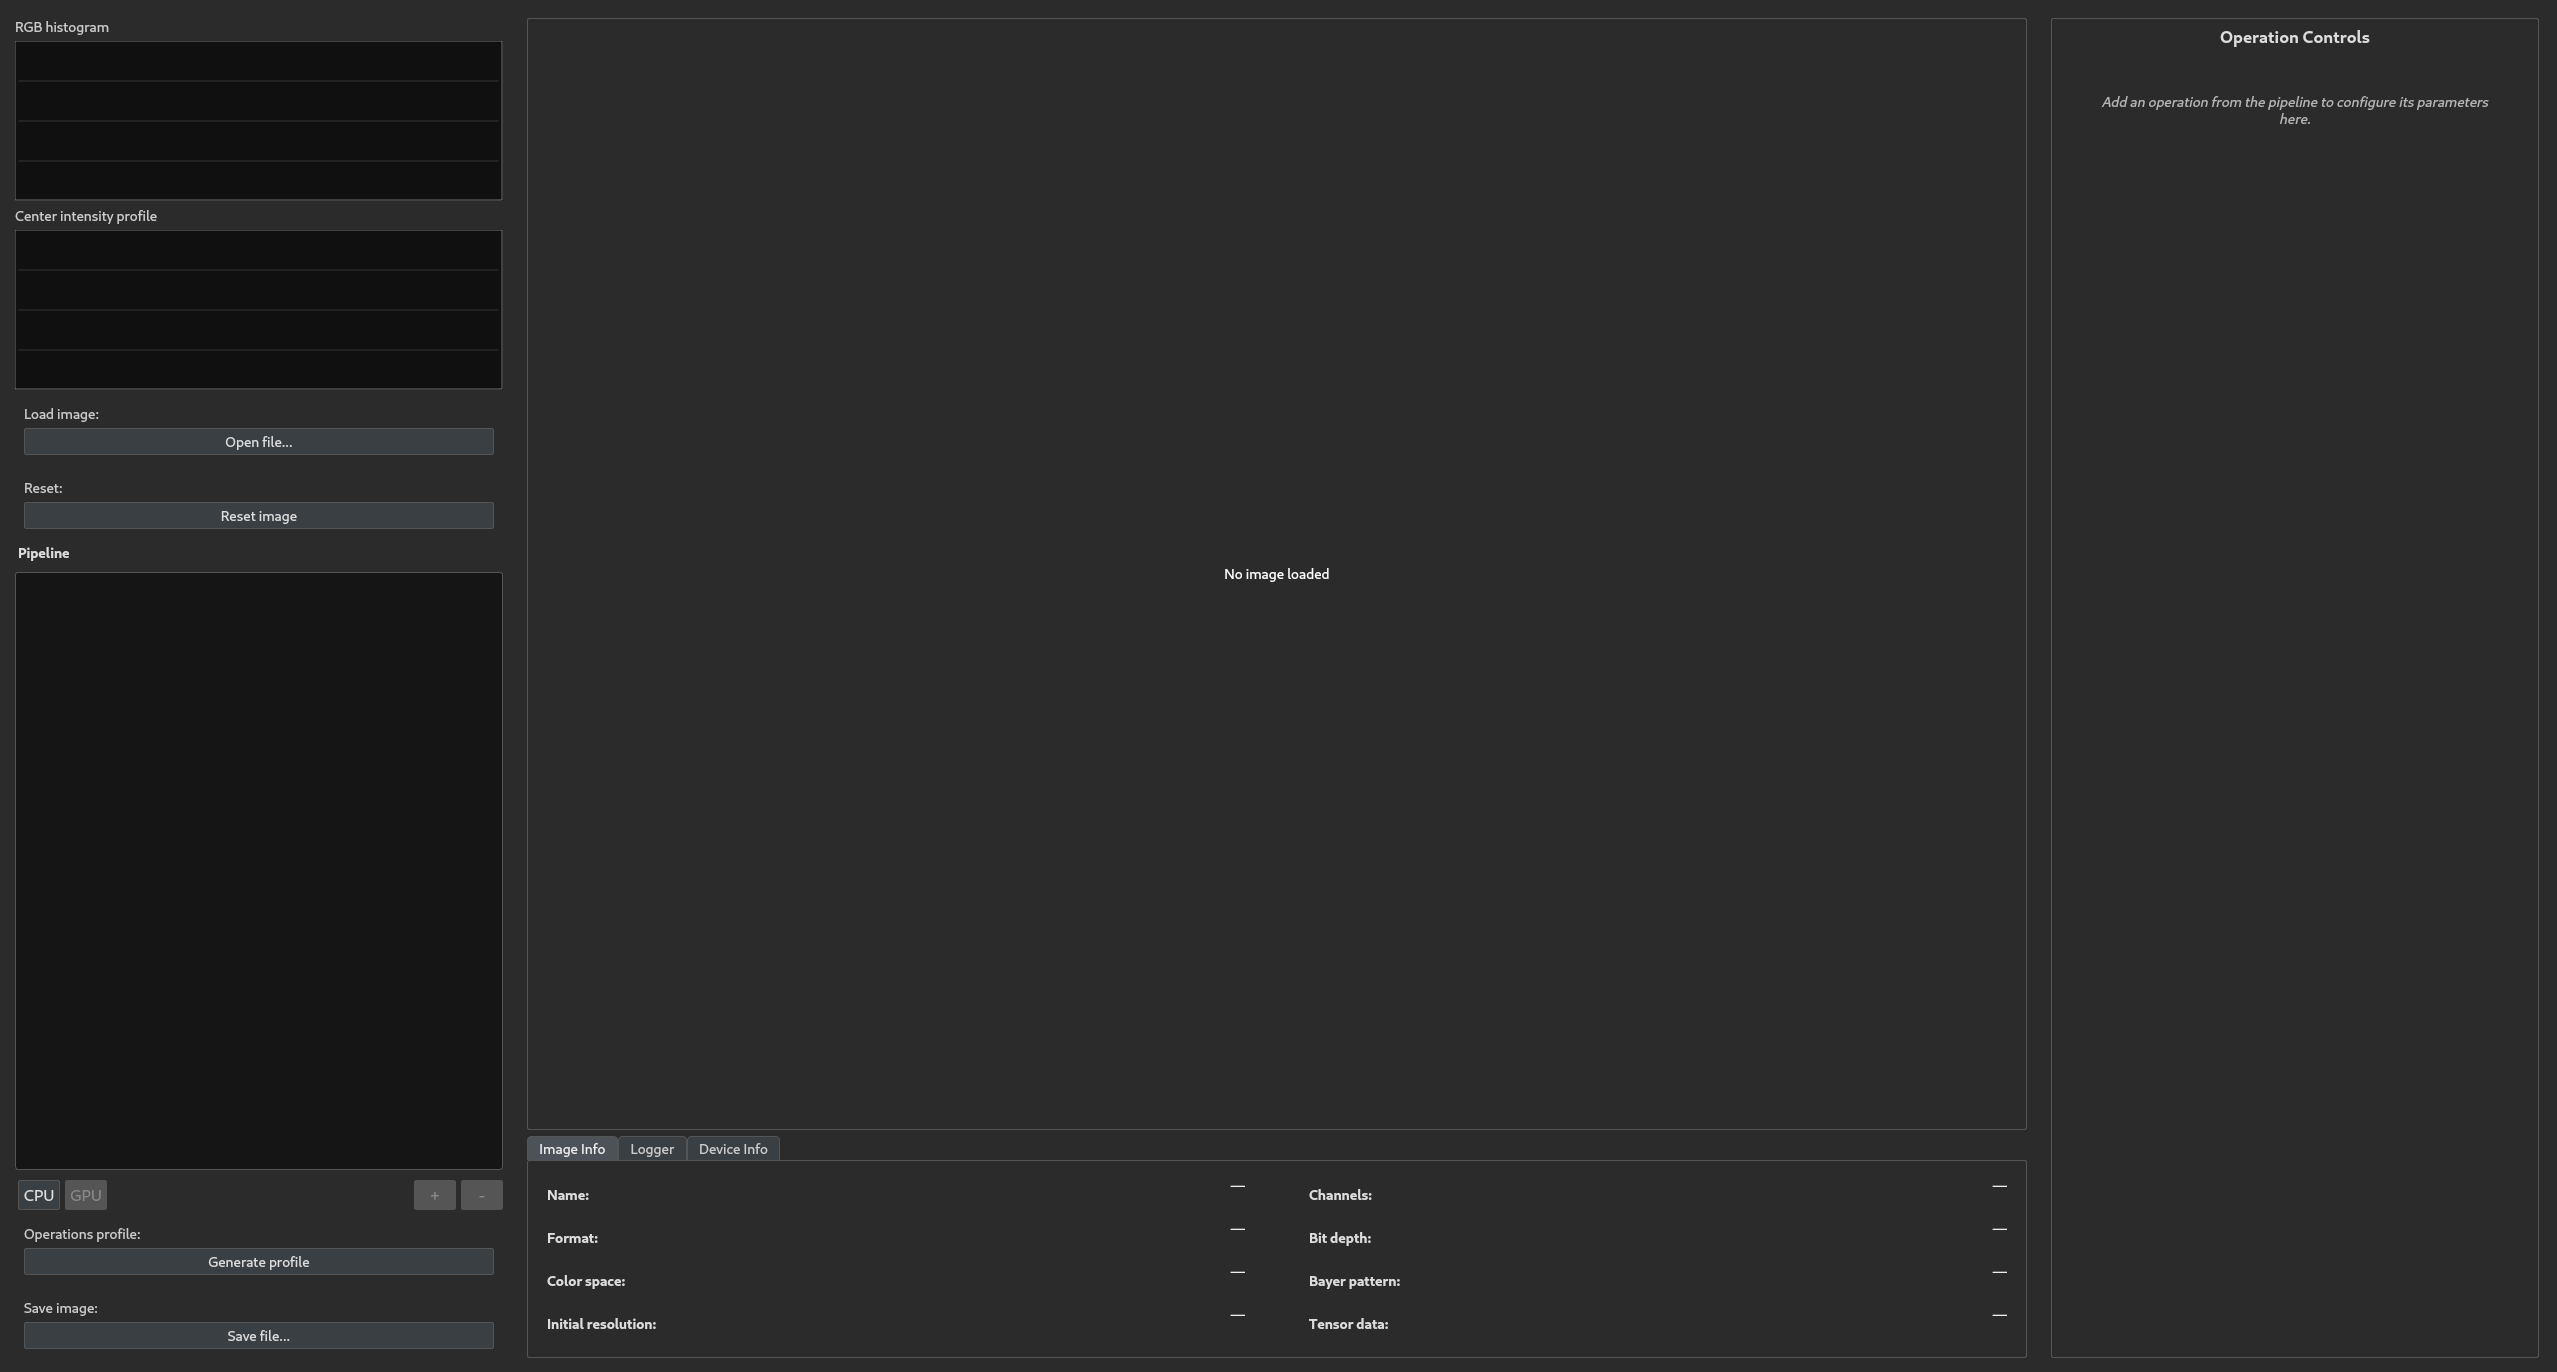
\includegraphics[width=0.8425\textwidth]{sections/7/img/gui_no_image_loaded.png}
    \caption{Visión general de la interfaz gráfica (sin imagen cargada)}
    \label{fig:35_gui_no_image_loaded_overview}
\end{figure}

\begin{figure}[h!]
    \centering
    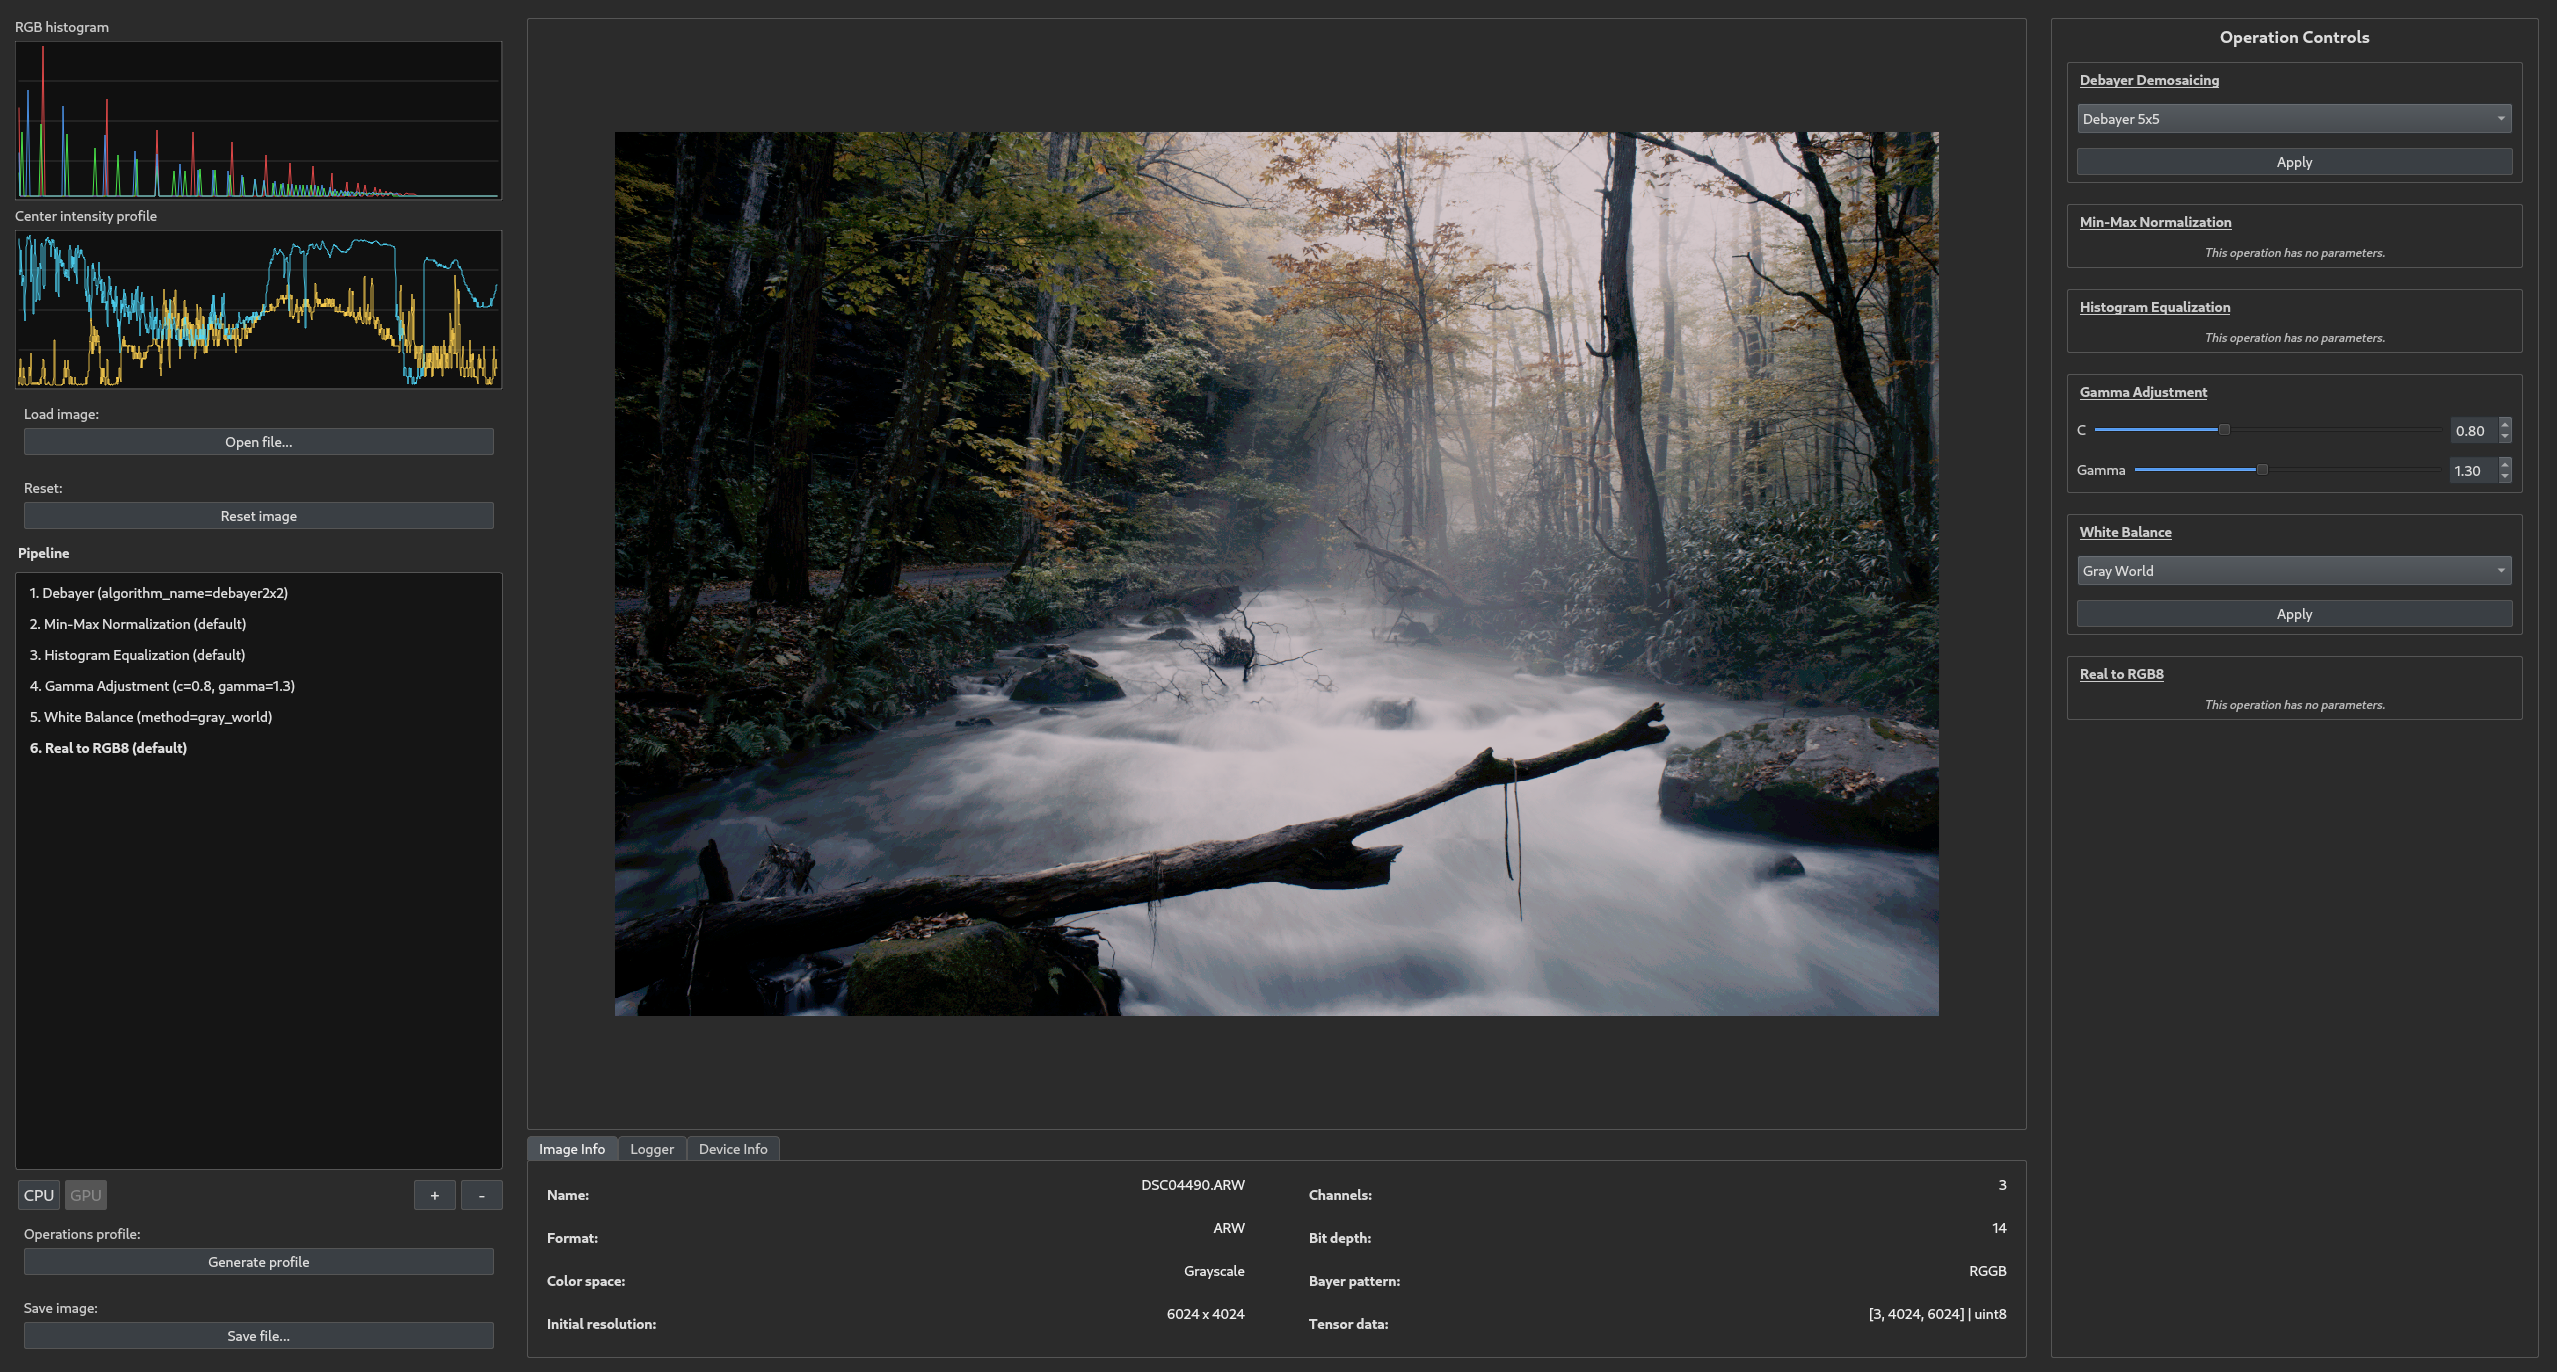
\includegraphics[width=0.8425\textwidth]{sections/7/img/gui_image_loaded.png}
    \caption{Visión general de la interfaz gráfica (con imagen cargada)}
    \label{fig:36_gui_image_loaded_overview}
\end{figure}

\newpage

\noindent{La interfaz se organiza en tres paneles principales distribuidos verticalmente:}

\begin{itemize}[noitemsep]
    \item \textbf{Panel izquierdo} (\texttt{LeftPanel})
    \item \textbf{Visor central} (\texttt{ImageViewer})
    \item \textbf{Panel derecho} (\texttt{RightPanel})
\end{itemize}

\paragraph{Panel izquierdo (\textit{LeftPanel})} \label{par:7_3_5_1_left_panel}
El panel izquierdo es el encargado de gestionar las principales acciones que se pueden realizar desde 
la interfaz gráfica. Actúa como centro de control. En la \autoref{fig:37_gui_left_panel_overview} se 
muestra su disposición respecto al resto de la interfaz.

\begin{figure}[h!]
    \centering
    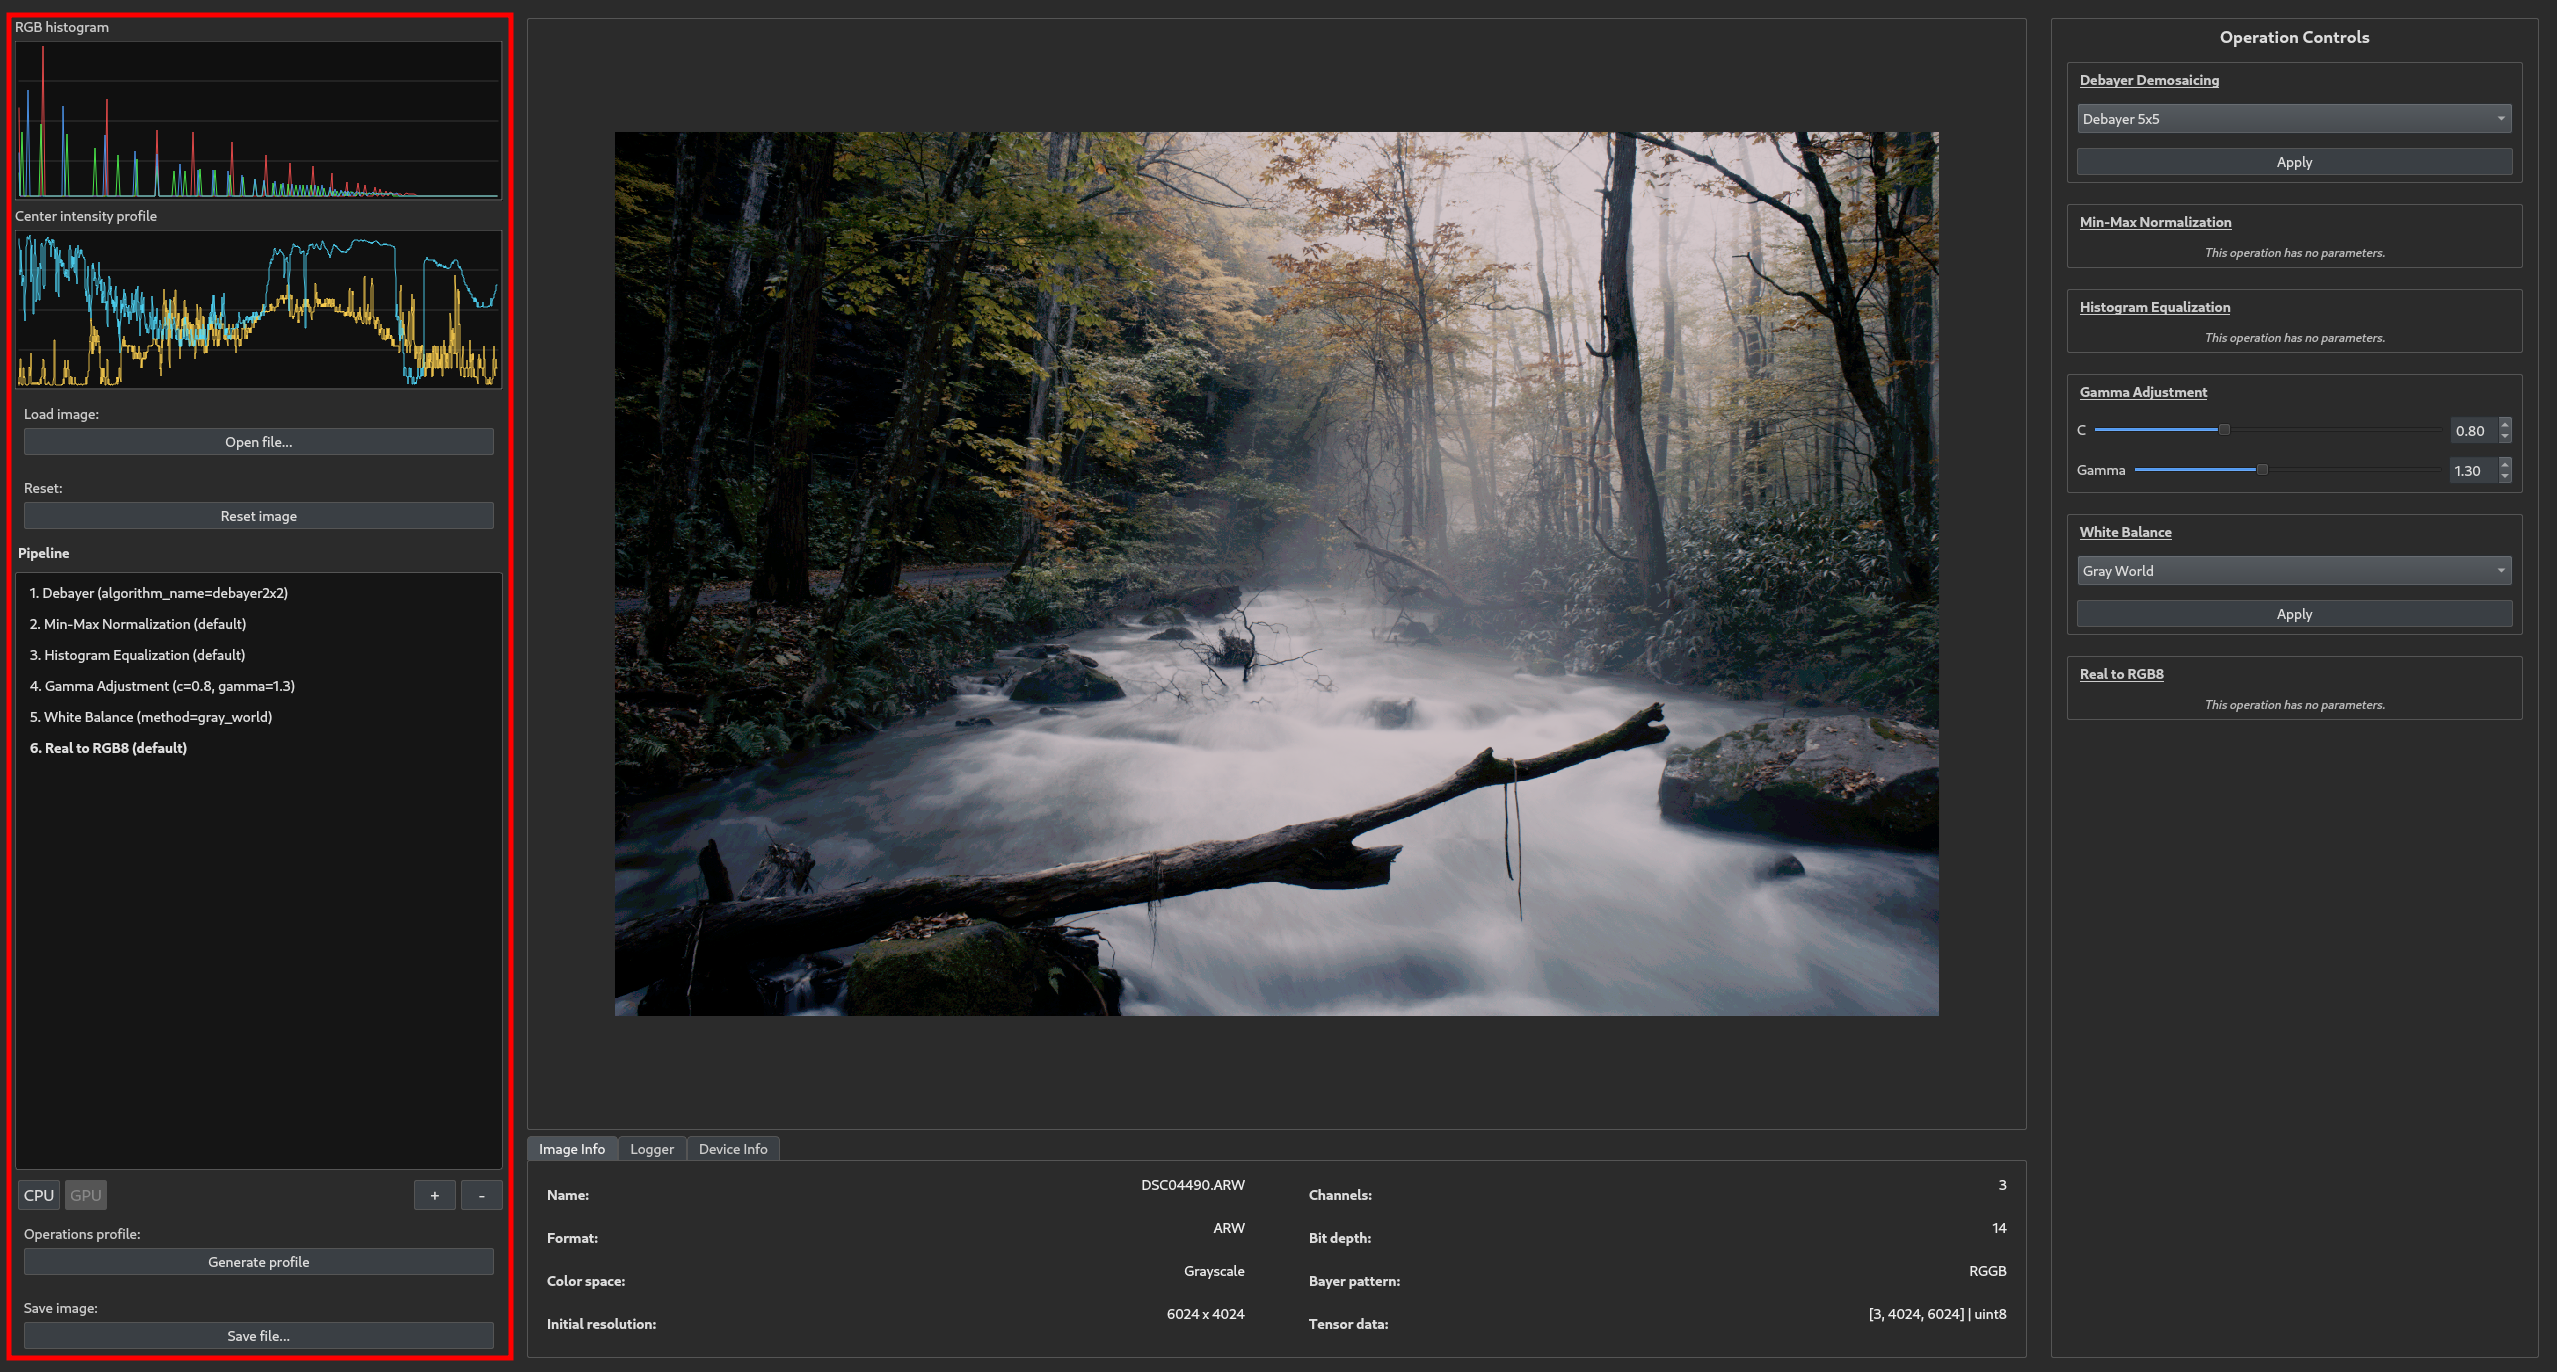
\includegraphics[width=0.8425\textwidth]{sections/7/img/gui_left_panel.png}
    \caption{Panel izquierdo (\textit{LeftPanel})}
    \label{fig:37_gui_left_panel_overview}
\end{figure}

\noindent
\begin{minipage}[t]{0.49\textwidth}
    \vspace{0pt}
    \setlength{\parindent}{2em}
    Los primeros elementos que renderiza este componente son dos gráficos que muestran 
    información de análisis sobre la imagen cargada, los cuales se muestran en la parte superior del panel.
    \begin{itemize}[noitemsep]
        \item \textbf{Histograma RGB}. Muestra la distribución de valores de píxeles para cada canal de color (\autoref{subsubsubsec:3_5_2_1_histograma}).
        \item \textbf{Perfiles centrales de intensidad}. Representa la intensidad de los perfiles vertical 
        y horizontal que atraviesan el centro de la imagen (\autoref{subsubsubsec:3_5_2_2_grafico_perfiles_intensidad}).
    \end{itemize}
    En la \autoref{fig:38_left_panel} se muestran dichos gráficos.
\end{minipage}\hfill
\begin{minipage}[t]{0.49\textwidth}
    \vspace{0pt}
    \centering
    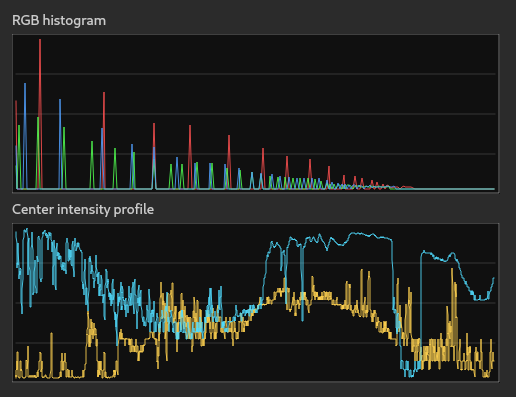
\includegraphics[width=0.8\linewidth]{sections/7/img/left_panel_plots.png}
    \captionsetup{justification=centering}
    \captionof{figure}{Gráficos de información \\ de la imagen}
    \label{fig:38_left_panel}
\end{minipage}

\newpage

\noindent
\begin{minipage}[t]{0.49\textwidth}
    \vspace{0pt}
    \setlength{\parindent}{2em}
    Justo debajo de los gráficos, se renderizan dos botones. El primero de ellos permite cargar una nueva imagen 
    completamente desde cero, mientras que el segundo restablece la imagen actual a su estado original, eliminando 
    todas las operaciones de procesamiento aplicadas. Dichos botones se muestran en la \autoref{fig:39_save_reset_buttons}.
    \vspace{1em}

    Tras estos botones, se renderiza uno de los componentes más importantes de la interfaz, el \textit{selector de operaciones}
    (\autoref{fig:40_pipeline_component}) para el \textit{pipeline} de procesamiento. Este componente permite añadir y eliminar 
    operaciones a la secuencia de procesamiento, mostrando una lista ordenada de las operaciones aplicadas y sus respectivos parámetros.
    Actúa como una pila: añade nuevas operaciones al final de la lista y permite eliminar la última operación aplicada. Esta pila se maneja 
    con los botones ``+'' y ``-'' ubicados en la parte inferior derecha del componente. El botón ``+'' despliega un menú con todas las operaciones
    disponibles, organizadas por categorías. Cada operación se aplica con sus parámetros por defecto, aunque el usuario puede modificarlos 
    posteriormente. Además, en la parte inferior izquierda del componente, se renderiza un botón de tipo \textit{toggle} [CPU/GPU] que permite 
    cambiar el dispositivo de procesamiento en el que se ejecutan las operaciones, mostrando el dispositivo seleccionado.
    \vspace{1em}

    Finalmente, en la parte inferior del panel izquierdo, se renderizan dos botones adicionales (\autoref{fig:41_op_profile_save_image_buttons}).
    El primero de ellos genera un perfil de ejecución en formato \textit{json} que representa el \textit{pipeline} de operaciones. Su 
    función es la exportación de la secuencia de operaciones aplicadas para su análisis en el módulo de \textit{benchmarking}. 
    El segundo botón permite guardar la imagen procesada en formato \textit{jpg}.
\end{minipage}\hfill
\begin{minipage}[t]{0.49\textwidth}
    \vspace{0pt}
    \centering
    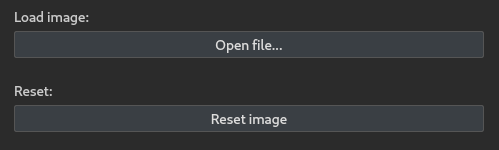
\includegraphics[width=0.85\textwidth]{sections/7/img/save_reset_buttons.png}
    \captionsetup{justification=centering}
    \captionof{figure}{Botones de guardado y \\ reinicio}
    \label{fig:39_save_reset_buttons}
    \vspace{2.25em}
    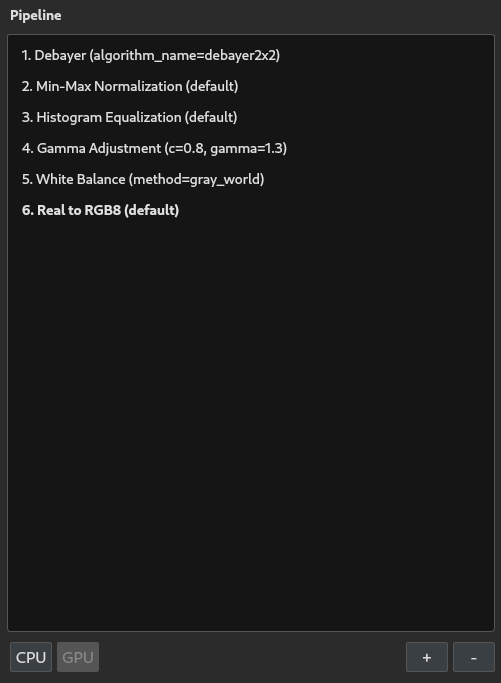
\includegraphics[width=0.85\linewidth]{sections/7/img/pipeline_component.png}
    \captionsetup{justification=centering}
    \captionof{figure}{Selector de operaciones}
    \label{fig:40_pipeline_component}
    \vspace{2.25em}
    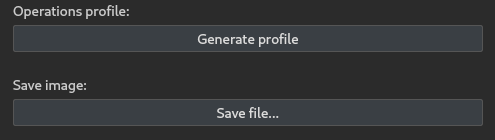
\includegraphics[width=0.85\linewidth]{sections/7/img/op_profile_save_image_buttons.png}
    \captionsetup{justification=centering}
    \captionof{figure}{Botones para generar el \\ perfil de ejecución de operaciones y \\ guardar la imagen procesada}
    \label{fig:41_op_profile_save_image_buttons}
\end{minipage}

\newpage

\paragraph{Visor central (\textit{ImageViewer})} \label{par:7_3_5_2_image_viewer}
El visor central es el componente principal de toda la interfaz. Es el encargado de mostrar la imagen cargada y procesada, actualizándose 
cada vez que se aplica una nueva operación o se lleva a cabo un ajuste de parámetros. Además, muestra información técnica sobre la imagen y 
el propio procesamiento. En la \autoref{fig:42_gui_image_viewer_overview} se muestra su disposición respecto al resto de la interfaz.

\begin{figure}[h!]
    \centering
    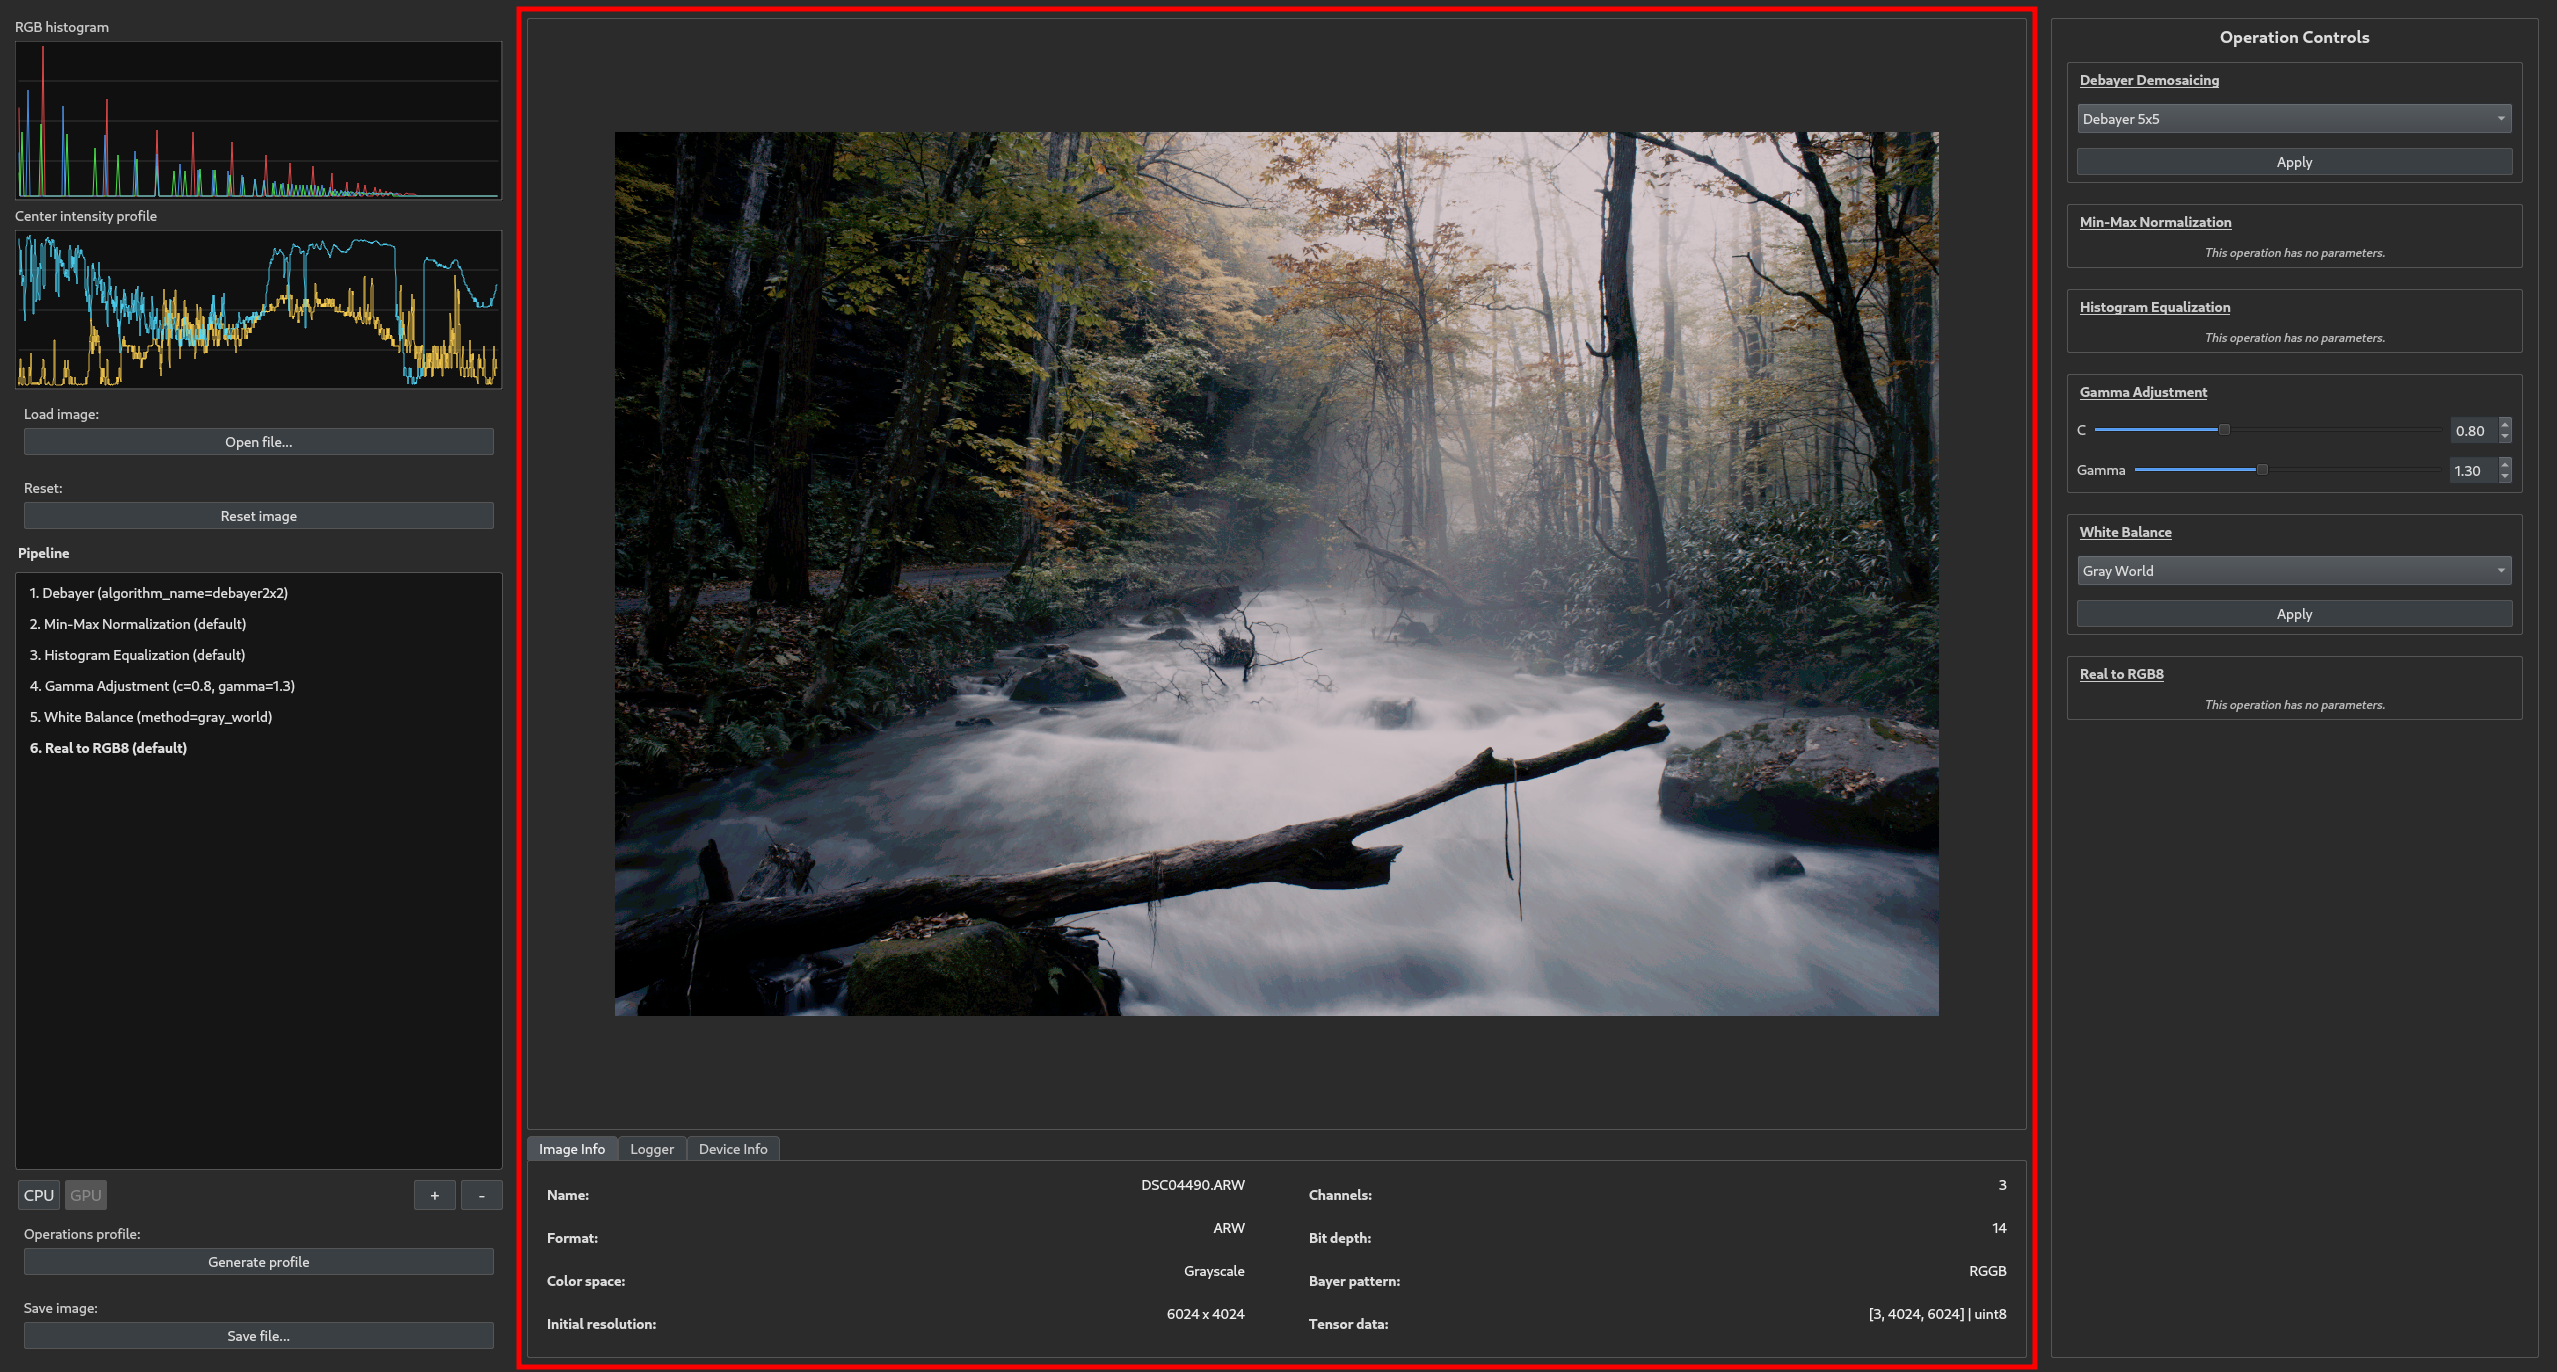
\includegraphics[width=0.8425\textwidth]{sections/7/img/gui_image_viewer.png}
    \caption{Visor central (\textit{ImageViewer})}
    \label{fig:42_gui_image_viewer_overview}
\end{figure}

Este componente se divide en dos partes claramente diferenciadas: un visor principal que muestra la imagen y una sección de \textit{tabs} 
inferior que muestra información. El visor principal permite, además de visualizar la imagen, realizar acciones de zoom y desplazamiento para facilitar 
la inspección de detalles. La sección de \textit{tabs} se organiza en tres pestañas: \textit{Image Info}, \textit{Logger} y \textit{Device Info}, como 
se puede observar en la \autoref{fig:43_image_info_tab_pane}.

\begin{figure}[h!]
    \centering
    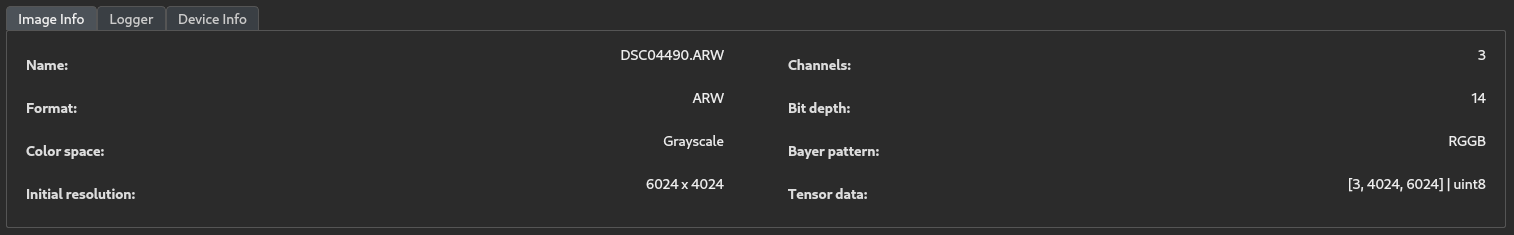
\includegraphics[width=0.9425\textwidth]{sections/7/img/image_info_tab_pane.png}
    \caption{Sección de \textit{tabs} del visor central}
    \label{fig:43_image_info_tab_pane}
\end{figure}

\noindent
La primera de las pestañas (\textit{Image Info}) muestra información técnica sobre la imagen cargada:
\vspace{-0.8em}
\begin{multicols}{2}
\begin{itemize}[noitemsep, topsep=0pt, parsep=0pt, partopsep=0pt]
    \item Nombre de la imagen
    \item Formato
    \item Espacio de color
    \item Dimensiones (ancho $\times$ alto)
    \item Número de canales
    \item Profundidad de bits
    \item Patrón Bayer (si aplica)
    \item Estado del tensor $\rightarrow$ [C, H, W] | Tipo de dato
\end{itemize}
\end{multicols}

\newpage

La segunda de las pestañas (\textit{Logger}) muestra un registro de eventos que representa todas las acciones realizadas por el usuario durante la sesión actual.
Esta pestaña tiene una función meramente informativa, proporcionando retroalimentación al usuario sobre las operaciones aplicadas, los cambios de parámetros, el dispositivo de procesamiento seleccionado, etc.
En la \autoref{fig:44_logger_tab_pane} se muestra un ejemplo de esta pestaña, que refleja el registro de acciones realizadas para la toma de las capturas de pantalla anteriores:
Carga de imagen $\rightarrow$ Aplicación de \textit{Debayer} $\rightarrow$ Aplicación de Normalización mín. máx. $\rightarrow$ Aplicación de Ecualización de Histograma $\rightarrow$ Aplicación de Ajuste \textit{Gamma}.
\begin{figure}[h!]
    \centering
    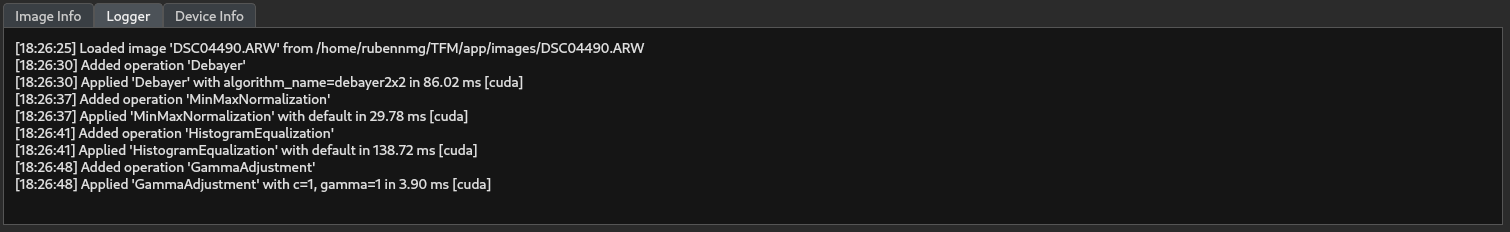
\includegraphics[width=0.98\textwidth]{sections/7/img/logger_tab_pane.png}
    \caption{Pestaña de \textit{Logger} del visor central}
    \label{fig:44_logger_tab_pane}
\end{figure}

Además, tras la aplicación de cada operación, se muestra el tiempo de ejecución en milisegundos, lo que permite obtener una primera referencia sobre el rendimiento de cada operación aplicada.
Como desde la propia aplicación se puede modificar el dispositivo de procesamiento (CPU o GPU), pueden hacerse pequeñas comparativas de rendimiento de forma sencilla e interactiva, lo 
que puede ser de gran utilidad. En la \autoref{fig:45_logger_cuda_cpu} se muestra un ejemplo de esta funcionalidad, donde se observa la aplicación de ciertas operaciones en ambos dispositivos 
de ejecución y los tiempos correspondientes.

\begin{figure}[h!]
    \centering
    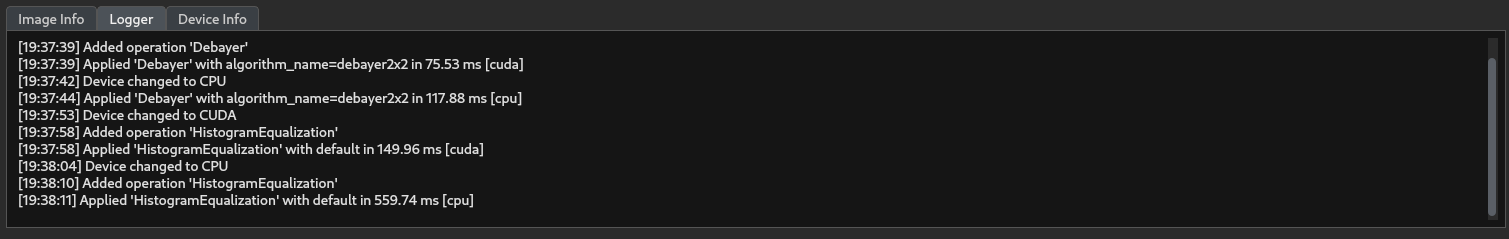
\includegraphics[width=0.98\textwidth]{sections/7/img/logger_cuda_cpu.png}
    \caption{Cambio de dispositivo de procesamiento y referencia de tiempos de ejecución}
    \label{fig:45_logger_cuda_cpu}
\end{figure}

Finalmente, la última de las pestañas (\textit{Device Info}) muestra información que \textit{PyTorch} proporciona sobre CUDA \cite{cuda} y 
las GPUs disponibles en el sistema, como puede observarse en la \autoref{fig:46_device_info_tab_pane}.

\begin{figure}[h!]
    \centering
    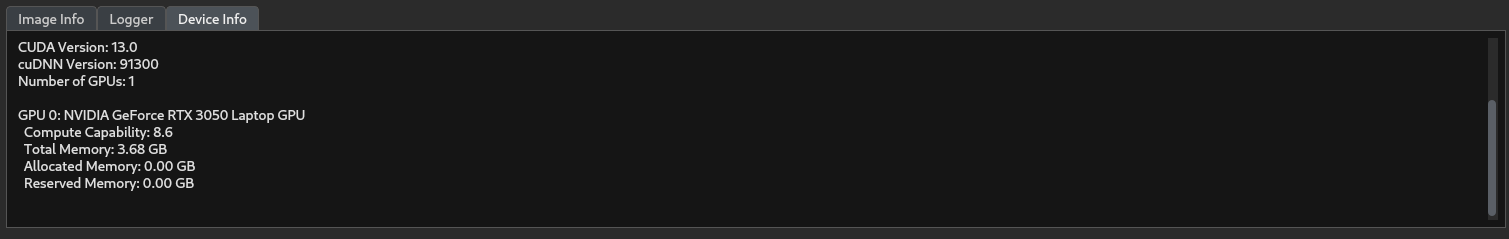
\includegraphics[width=0.98\textwidth]{sections/7/img/device_info_tab_pane.png}
    \caption{Pestaña de \textit{Device Info} del visor central}
    \label{fig:46_device_info_tab_pane}
\end{figure}

\newpage

\paragraph{Panel derecho (\textit{RightPanel})} \label{par:7_3_5_3_right_panel}
El panel derecho se encarga de renderizar controles sobre las operaciones aplicadas desde el panel izquierdo para modificar
y ajustar sus parámetros. Cada vez que se añade una nueva operación al \textit{pipeline} de procesamiento, se añade 
un control específico para dicha operación en el panel derecho. En la \autoref{fig:47_gui_right_panel_overview} 
se muestra su disposición respecto al resto de la interfaz, así como un ejemplo de los controles renderizados 
para un \textit{pipeline} específico.

\begin{figure}[h!]
    \centering
    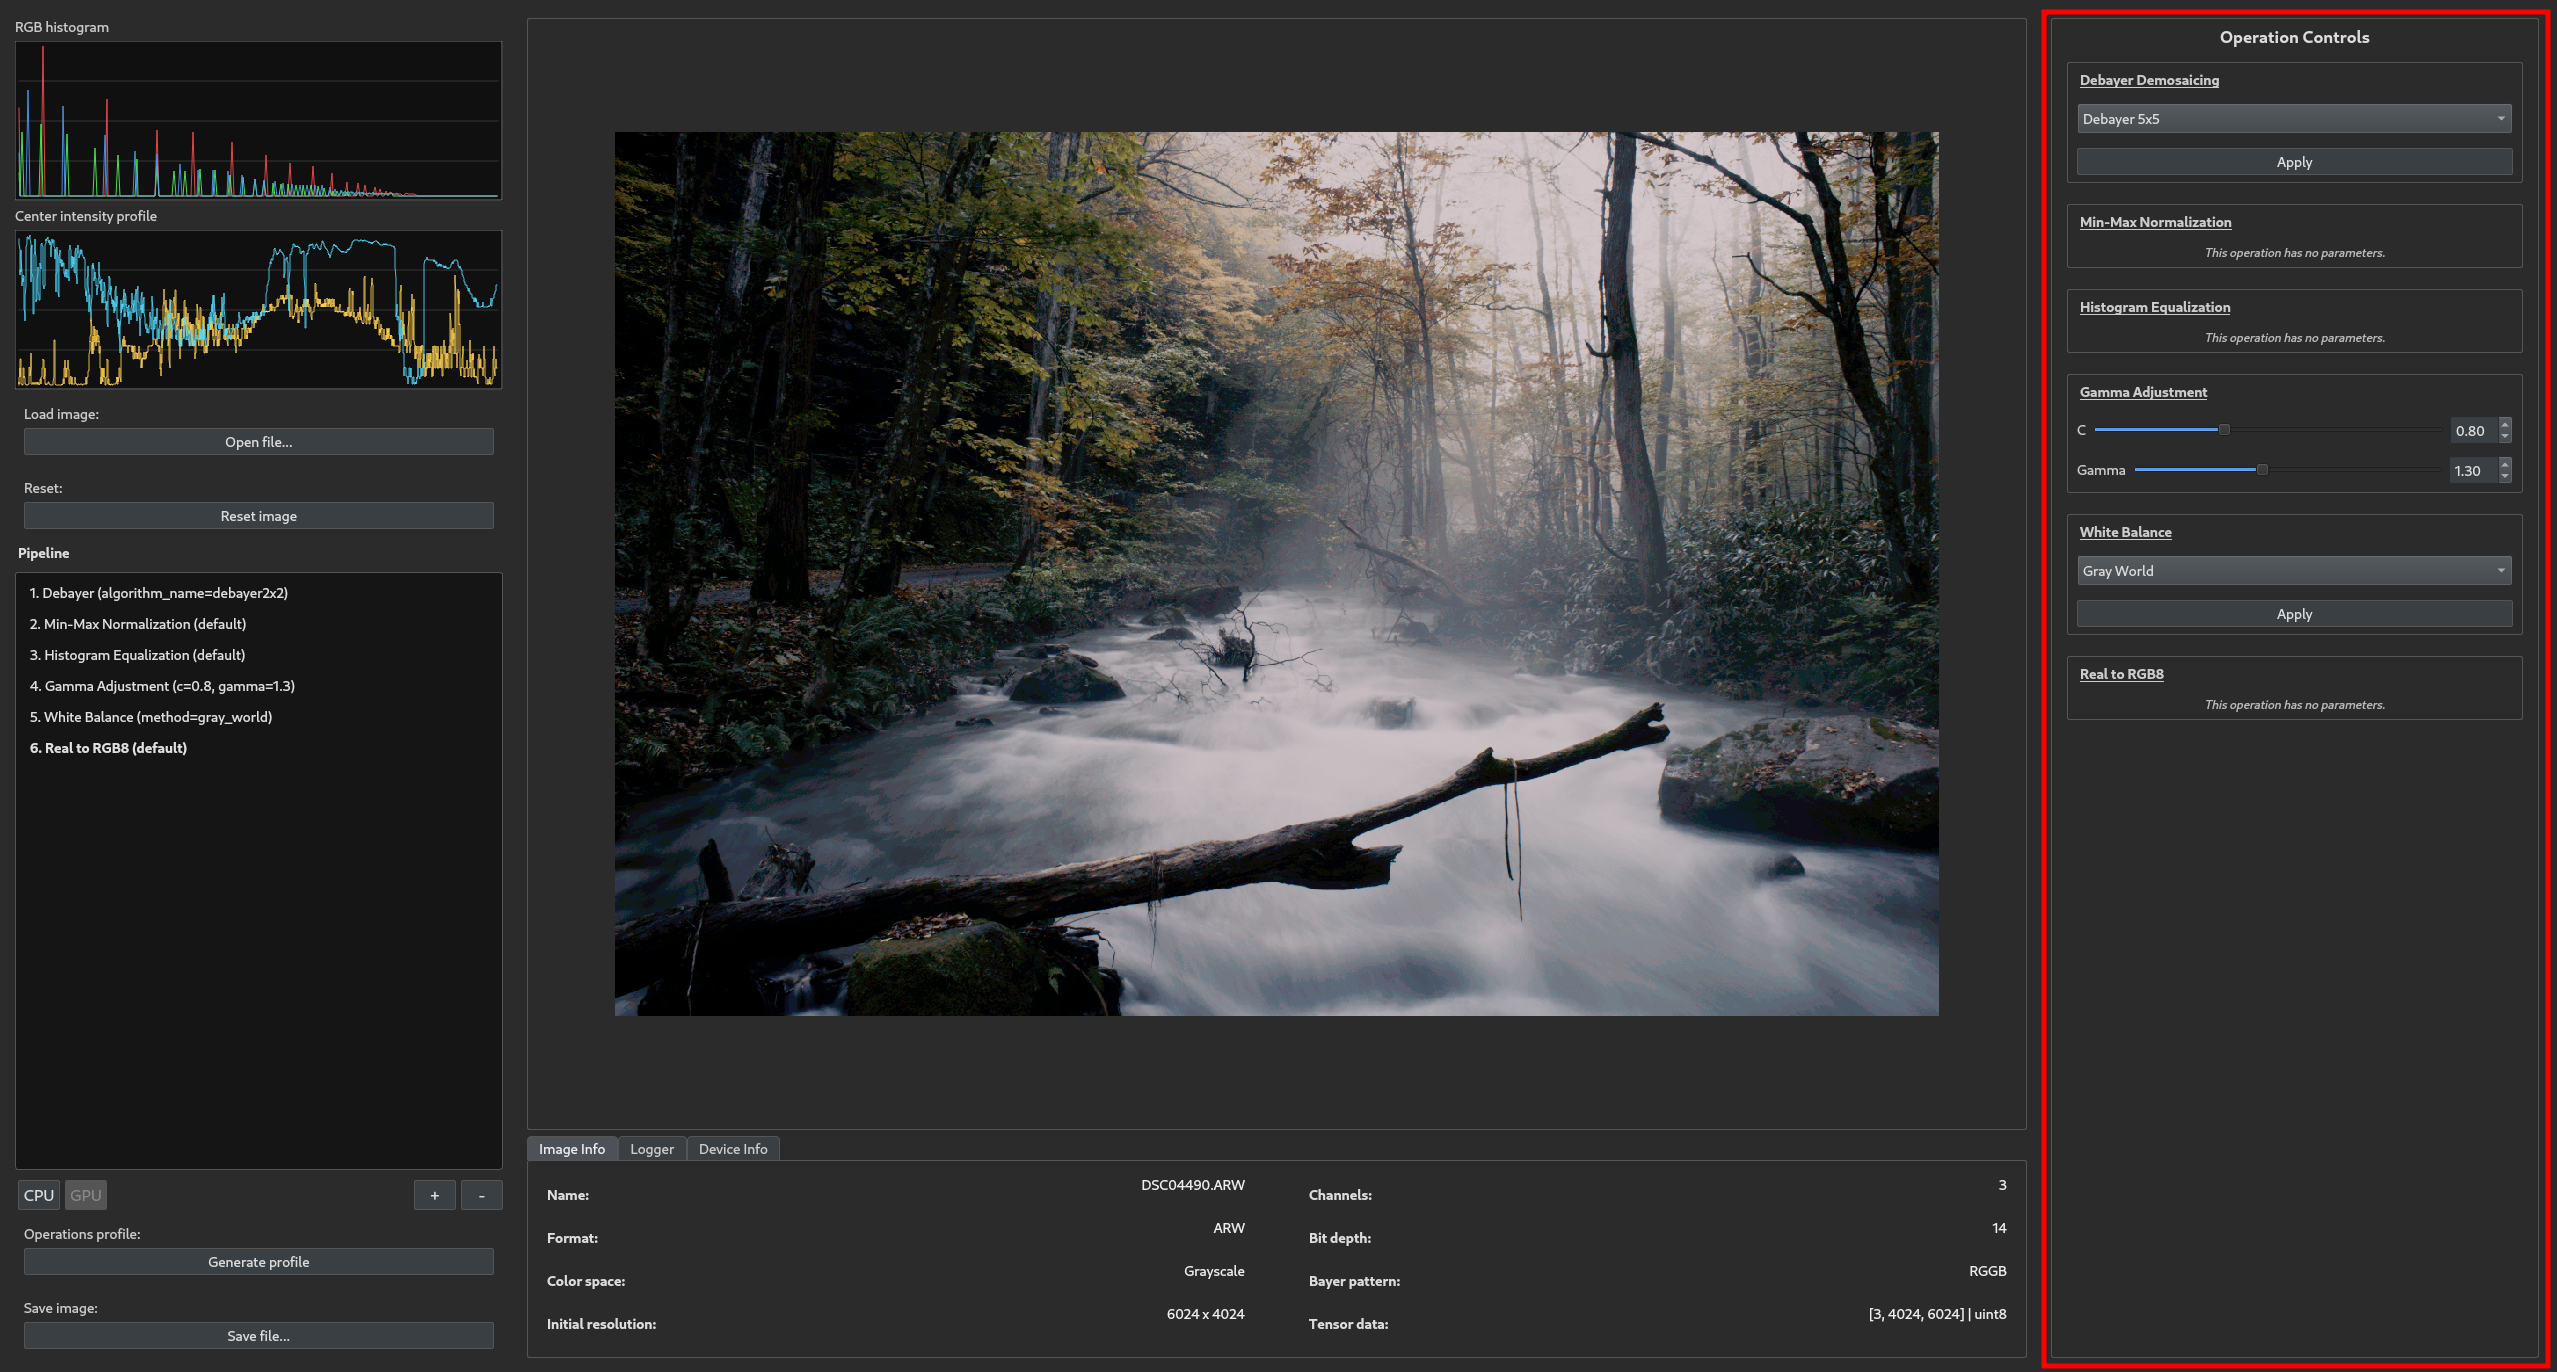
\includegraphics[width=0.8425\textwidth]{sections/7/img/gui_right_panel.png}
    \caption{Panel derecho (\textit{RightPanel})}
    \label{fig:47_gui_right_panel_overview}
\end{figure}

Desde estos controles, el usuario puede modificar los parámetros de cada operación aplicada, independientemente 
del orden en el que se encuentren en el \textit{pipeline}. Como cada operación tiene sus propios parámetros, 
se han desarrollado diferentes tipos de controles para cada caso.

El primer tipo de control es el específico para operaciones que requieren la selección de tipo de algoritmo o método 
a aplicar, esto es, una selección entre varias opciones predefinidas. Este es el caso de la operación \textit{Debayer}, que 
tiene diferentes módulos implementados, y de la operación de Balance de Blancos (\textit{White Balance}), que permite la 
selección entre diferentes algoritmos. Dicho control muestra un simple menú desplegable de tipo \textit{dropdown} con las opciones 
disponibles para cada operación, como se muestra en la \autoref{fig:48_op_controls_method_selection}.

\begin{figure}[h!]
    \centering
    \begin{subfigure}{0.49\textwidth}
        \centering
        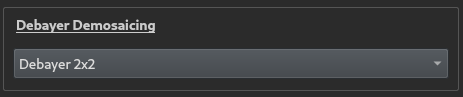
\includegraphics[width=0.925\textwidth]{sections/7/img/debayer_op_control.png}
        \caption{Control para operación \textit{Debayer}}
        \label{fig:48_a_debayer_op_control}
    \end{subfigure}\hfill
    \begin{subfigure}{0.49\textwidth}
        \centering
        
\includegraphics[width=0.925\textwidth]{sections/7/img/white_balance_op_control.png}
        \caption{Control para operación \textit{White Balance}}
        \label{fig:48_b_white_balance_op_control}
    \end{subfigure}
    \caption{Controles para operaciones con selección de método o algoritmo}
    \label{fig:48_op_controls_method_selection}
\end{figure}

\newpage

Otro tipo de control es el específico para operaciones que requieren la modificación de uno o varios parámetros numéricos.
En este caso, se renderizan de forma dinámica elementos de tipo \textit{slider} o \textit{spinbox} para cada parámetro 
de la operación, permitiendo su ajuste de forma interactiva. Cada cambio en cualquiera de estos elementos implica la 
actualización inmediata de la imagen en el visor central, mostrando el resultado del ajuste. En la \autoref{fig:49_op_controls_filters}
se muestran todas las operaciones que utilizan este tipo de control.

\begin{figure}[h!]
    \centering
    \begin{subfigure}{0.49\textwidth}
        \centering
        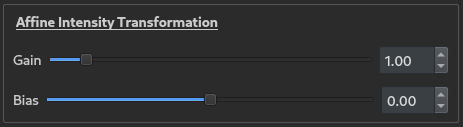
\includegraphics[width=0.925\textwidth]{sections/7/img/affine_intensity_transformation_op_control.png}
        \caption{Control para Ajuste de Intensidad Afín}
        \label{fig:49_a_affine_intensity_transformation_op_control}
    \end{subfigure}\hfill
    \begin{subfigure}{0.49\textwidth}
        \centering
        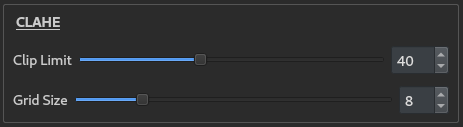
\includegraphics[width=0.925\textwidth]{sections/7/img/clahe_op_control.png}
        \caption{Control para \textit{CLAHE}}
        \label{fig:49_b_clahe_op_control}
    \end{subfigure}
    \\[1em]
    \begin{subfigure}{0.49\textwidth}
        \centering
        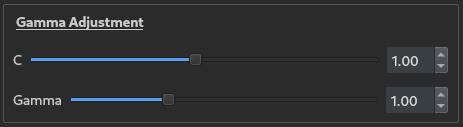
\includegraphics[width=0.925\textwidth]{sections/7/img/gamma_adjustment_op_control.png}
        \caption{Control para Ajuste \textit{Gamma}}
        \label{fig:49_c_gamma_adjustment_op_control}
    \end{subfigure}\hfill
    \begin{subfigure}{0.49\textwidth}
        \centering
        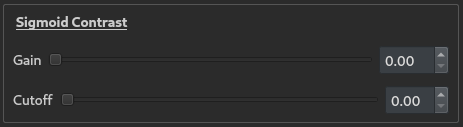
\includegraphics[width=0.925\textwidth]{sections/7/img/sigmoid_contrast_op_control.png}
        \caption{Control para Ajuste de Contraste mediante Sigmoide}
        \label{fig:49_d_sigmoid_contrast_op_control}
    \end{subfigure}
    \\[1em]
    \begin{subfigure}{0.49\textwidth}
        \centering
        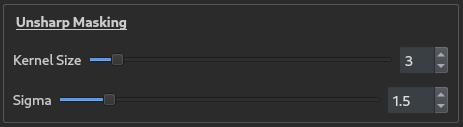
\includegraphics[width=0.925\textwidth]{sections/7/img/unsharp_masking_op_control.png}
        \caption{Control para \textit{Unsharp Masking}}
        \label{fig:49_e_unsharp_masking_op_control}
    \end{subfigure}\hfill
    \begin{subfigure}{0.49\textwidth}
        \centering
        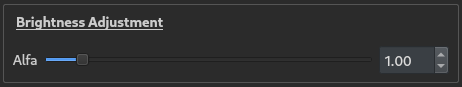
\includegraphics[width=0.925\textwidth]{sections/7/img/brightness_adjustment_op_control.png}
        \caption{Control para Ajuste de Brillo}
        \label{fig:49_f_brightness_adjustment_op_control}
    \end{subfigure}
    \\[1em]
    \begin{subfigure}{0.49\textwidth}
        \centering
        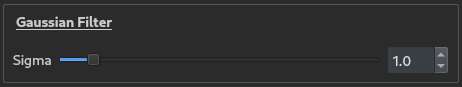
\includegraphics[width=0.925\textwidth]{sections/7/img/gaussian_filter_op_control.png}
        \caption{Control para Filtro Gaussiano}
        \label{fig:49_g_gaussian_filter_op_control}
    \end{subfigure}\hfill
    \begin{subfigure}{0.49\textwidth}
        \centering
        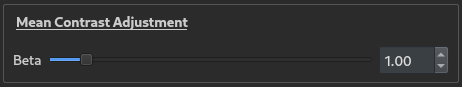
\includegraphics[width=0.925\textwidth]{sections/7/img/mean_contrast_adjustment_op_control.png}
        \caption{Control para Ajuste de Contraste}
        \label{fig:49_h_mean_contrast_adjustment_op_control}
    \end{subfigure}
    \\[1em]
    \begin{subfigure}{0.49\textwidth}
        \centering
        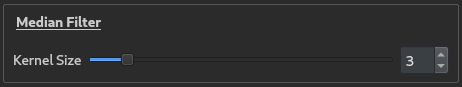
\includegraphics[width=0.925\textwidth]{sections/7/img/median_filter_op_control.png}
        \caption{Control para Filtro de Mediana}
        \label{fig:49_i_median_filter_op_control}
    \end{subfigure}\hfill
    \begin{subfigure}{0.49\textwidth}
        \centering
        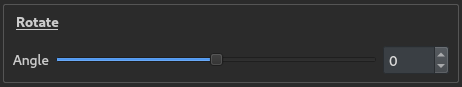
\includegraphics[width=0.925\textwidth]{sections/7/img/rotate_op_control.png}
        \caption{Control para Rotación de imagen}
        \label{fig:49_j_rotate_op_control}
    \end{subfigure}
    \caption{Controles para operaciones con parámetros numéricos ajustables}
    \label{fig:49_op_controls_filters}
\end{figure}

\newpage

Similar al caso anterior, se implementa otro tipo de control para operaciones que requieren la modificación de dos parámetros
numéricos para un rango de valores. Este es el caso de las operaciones mostradas en la 
\autoref{fig:50_numeric_spin_op_controls}. Estos controles renderizan dos elementos de tipo \textit{spinbox} para cada 
parámetro, permitiendo su ajuste de forma interactiva.

\begin{figure}[h!]
    \centering
    \begin{subfigure}{0.49\textwidth}
        \centering
        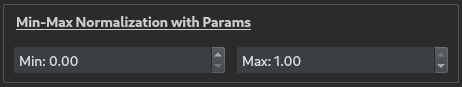
\includegraphics[width=0.925\textwidth]{sections/7/img/min_max_with_params_op_control.png}
        \caption{Control para Normalización con parámetros}
        \label{fig:50_a_min_max_with_params_op_control}
    \end{subfigure}
    \\[1.5em]
    \begin{subfigure}{0.49\textwidth}
        \centering
        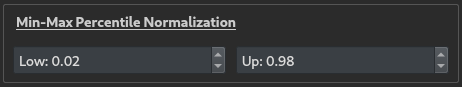
\includegraphics[width=0.925\textwidth]{sections/7/img/min_max_percentile_op_control.png}
        \caption{Control para Normalización con percentiles}
        \label{fig:50_b_min_max_percentile_op_control}
    \end{subfigure}
    \hfill
    \begin{subfigure}{0.49\textwidth}
        \centering
        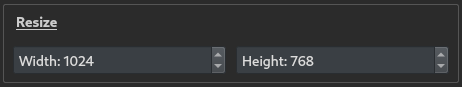
\includegraphics[width=0.925\textwidth]{sections/7/img/resize_op_control.png}
        \caption{Control para Redimensionamiento}
        \label{fig:50_c_resize_op_control}
    \end{subfigure}
    \caption{Controles para operaciones con parámetros numéricos ajustables (continuación)}
    \label{fig:50_numeric_spin_op_controls}
\end{figure}

Otras operaciones requieren otros tipos de parámetros, por lo que se han desarrollado otros controles específicos. Este 
es el caso de la operación de volteo de imagen (\textit{Flip}), que requiere el \textit{toggle} entre dos opciones (volteo
horizontal o vertical). Como puede observarse en la \autoref{fig:51_flip_op_control}, este control renderiza un \textit{radio button}
que permite seleccionar entre ambas opciones.

\begin{figure}[h!]
    \centering
    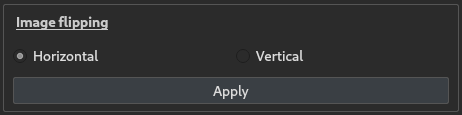
\includegraphics[width=0.45\textwidth]{sections/7/img/flip_op_control.png}
    \caption{Control para Volteo de imagen}
    \label{fig:51_flip_op_control}
\end{figure}

Otro caso es el de la operación de Compensación de Iluminación (\textit{Light Compensation}), que requiere la carga 
de un fichero \textit{npy} para especificar la matriz de compensación y el ajuste de un parámetro numérico para 
la intensidad. Para manejar esta operación, se desarrolla el control mostrado en la \autoref{fig:52_light_compensation_op_control}, 
que renderiza un botón para cargar el fichero de compensación y un \textit{slider} para ajustar la intensidad de la compensación aplicada a la imagen.

\begin{figure}[h!]
    \centering
    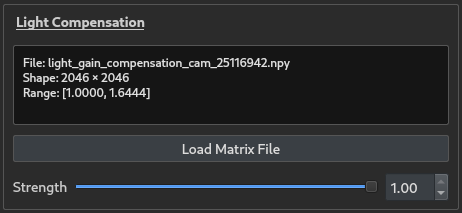
\includegraphics[width=0.45\textwidth]{sections/7/img/light_compensation_op_control.png}
    \caption{Control para Compensación de Iluminación}
    \label{fig:52_light_compensation_op_control}
\end{figure}

\newpage

Finalmente, existen operaciones que no requieren ningún tipo de parámetro, simplemente su aplicación implica la ejecución de 
un proceso específico sobre la imagen, como puede ser el caso de una conversión de formato o espacio de color, etc. 
Para este tipo de operaciones, se renderiza un control muy simple que muestra el nombre de la operación aplicada y un texto 
informativo que indica que no requiere ningún parámetro, como se muestra en la \autoref{fig:53_op_controls_no_param}.

\begin{figure}[h!]
    \centering
    \begin{subfigure}{0.49\textwidth}
        \centering
        
\includegraphics[width=0.925\textwidth]{sections/7/img/no_param_op_control/color_to_grayscale_op_control.png}
        \caption{Control para Conversión a Escala de Grises}
        \label{fig:53_a_color_to_grayscale_op_control}
    \end{subfigure}\hfill
    \begin{subfigure}{0.49\textwidth}
        \centering
        
\includegraphics[width=0.925\textwidth]{sections/7/img/no_param_op_control/grayscale_to_color_op_control.png}
        \caption{Control para Conversión a Color}
        \label{fig:53_b_grayscale_to_color_op_control}
    \end{subfigure}
    \\[1em]
    \begin{subfigure}{0.49\textwidth}
        \centering
        
\includegraphics[width=0.925\textwidth]{sections/7/img/no_param_op_control/histogram_equalization_op_control.png}
        \caption{Control para Ecualización de Histograma}
        \label{fig:53_c_histogram_equalization_op_control}
    \end{subfigure}\hfill
    \begin{subfigure}{0.49\textwidth}
        \centering
        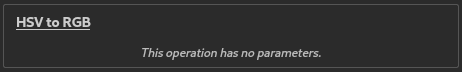
\includegraphics[width=0.925\textwidth]{sections/7/img/no_param_op_control/hsv_to_rgb_op_control.png}
        \caption{Control para Conversión HSV a RGB}
        \label{fig:53_d_hsv_to_rgb_op_control}
    \end{subfigure}
    \\[1em]
    \begin{subfigure}{0.49\textwidth}
        \centering
        
\includegraphics[width=0.925\textwidth]{sections/7/img/no_param_op_control/rgb_to_hsv_op_control.png}
        \caption{Control para Conversión RGB a HSV}
        \label{fig:53_e_rgb_to_hsv_op_control}
    \end{subfigure}\hfill
    \begin{subfigure}{0.49\textwidth}
        \centering
        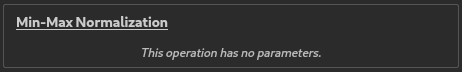
\includegraphics[width=0.925\textwidth]{sections/7/img/no_param_op_control/min_max_normalization_op_control.png}
        \caption{Control para Normalización mín. máx. \footnotemark}
        \label{fig:53_f_min_max_normalization_op_control}
    \end{subfigure}
    \\[1em]
    \begin{subfigure}{0.49\textwidth}
        \centering
        
\includegraphics[width=0.925\textwidth]{sections/7/img/no_param_op_control/rgb8_to_real_op_control.png}
        \caption{Control para Conversión RGB8 a Real}
        \label{fig:53_g_rgb8_to_real_op_control}
    \end{subfigure}\hfill
    \begin{subfigure}{0.49\textwidth}
        \centering
        
\includegraphics[width=0.925\textwidth]{sections/7/img/no_param_op_control/real_to_rgb8_op_control.png}
        \caption{Control para Conversión Real a RGB8}
        \label{fig:53_h_real_to_rgb8_op_control}
    \end{subfigure}
    \caption{Controles para operaciones sin parámetros}
    \label{fig:53_op_controls_no_param}
\end{figure}

\footnotetext{La operación de Normalización mín. máx. (\autoref{fig:53_f_min_max_normalization_op_control}) sin parámetros se
corresponde con la aplicación de esta técnica utilizando el valor mínimo y máximo de la imagen como parámetros, es decir, 
sin especificar manualmente ningún valor. Esta operación también puede aplicarse especificando manualmente los parámetros de 
mínimo y máximo, lo que se corresponde con la operación mostrada en la \autoref{fig:50_a_min_max_with_params_op_control}.}

\newpage

\subsubsection{Benchmark} \label{subsubsec:7_3_6_benchmark}
El componente \textit{Benchmark} se encarga de medir y analizar el rendimiento de los \textit{pipelines} de operaciones 
definidos por el usuario desde la \textit{GUI}. Su implementación se basa en \textit{pytest} \cite{pytest} y en el 
\textit{plugin} \textit{pytest-benchmark} \cite{pytest_benchmark}, lo que permite ejecutar medidas de rendimiento de forma repetitiva y
con salida estructurada en formato \textit{json}.

\paragraph{Arquitectura interna} \label{par:7_3_6_1_arquitectura_interna_benchmark}
El módulo se organiza alrededor de dos piezas principales: un archivo de configuración
(\textit{benchmark/conftest.py}) y un archivo de ejecución de pruebas de rendimiento
(\textit{benchmark/run.py}). Esta organización es típica de \textit{pytest} y permite separar la configuración 
general del \textit{benchmark} de la lógica específica de ejecución. Las funcionalidades clave del módulo incluyen:

\begin{itemize}[noitemsep]
    \item \textbf{Configuración global del \textit{benchmark}.} En \texttt{conftest.py} se definen
    parámetros comunes de ejecución (unidad temporal en milisegundos, \textit{warmup} activo,
    criterio de ordenación y tiempo máximo por caso).
    \item \textbf{Perfil de ejecución externo.} El módulo añade el argumento de línea de comandos
    \texttt{-{}-bench-profile}, que recibe la ruta de un fichero \textit{json} con la definición del
    \textit{pipeline} a evaluar.
    \item \textbf{Construcción dinámica del \textit{pipeline}.} Mediante una \textit{fixture}
    (\texttt{pipeline\_factory}), cada entrada del perfil se transforma en una instancia real de
    operación utilizando el registro global de operaciones (\texttt{OPERATION\_REGISTRY}, \autoref{par:7_3_3_2_sistema_registro}).
    \item \textbf{Matriz experimental parametrizada.} En \texttt{run.py}, el \textit{benchmark}
    se ejecuta para múltiples combinaciones de dispositivo de procesamiento, tamaño de imagen y tipo de dato,
    permitiendo comparar rendimiento y coste computacional en diferentes escenarios.
\end{itemize}

\paragraph{Flujo técnico de ejecución} \label{par:7_3_6_2_flujo_tecnico_benchmark}
\noindent{Para cada caso de la matriz experimental definida, el flujo es el siguiente:}

\begin{enumerate}[noitemsep]
    \item Carga y validación del perfil \textit{json} recibido por \texttt{-{}-bench-profile}, que representa el \textit{pipeline} de operaciones a evaluar.
    \item Resolución de operaciones por nombre a través de \texttt{OPERATION\_REGISTRY}.
    \item Instanciación de cada operación con sus parámetros.
    \item Construcción de una función \textit{pipeline} que aplica secuencialmente todas las operaciones recogidas en el mismo.
    \item Generación de un tensor sintético de entrada con las dimensiones y precisión numérica configuradas.
    \item Ejecución repetida del \textit{pipeline} mediante \textit{pytest-benchmark} para obtener métricas temporales.
    \item Persistencia de resultados en el directorio \texttt{.benchmarks/} para su análisis posterior.
\end{enumerate}

\newpage

\paragraph{Comunicación con el resto de la aplicación} \label{par:7_3_6_3_comunicacion_benchmark}
El componente \textit{Benchmark} es un componente especial porque no forma parte del flujo de ejecución normal de la aplicación interactiva, 
sino que se ejecuta de forma autónoma. 
La integración de dicho componente con el sistema completo se realiza mediante dos
mecanismos: un contrato de datos compartido y la reutilización del mismo núcleo \textit{Core} de operaciones. Dicha integración 
se basa en los siguientes principios:

\begin{itemize}[noitemsep]
    \item \textbf{Interfaz de intercambio (GUI $\leftrightarrow$ Benchmark).}
    Desde la interfaz gráfica, el usuario exporta el \textit{pipeline} actual; el \textit{Controller}
    lo serializa como una lista ordenada de operaciones y parámetros en formato \textit{json}.
    Ese fichero se convierte en la entrada directa del módulo \textit{Benchmark}.
    \item \textbf{Consistencia funcional (Core compartido).}
    El \textit{Benchmark} no reimplementa operaciones: instancia exactamente las mismas clases
    del componente \textit{Core} usando \texttt{OPERATION\_REGISTRY}. Lo que se mide es exactamente el mismo
    comportamiento que se ejecuta en la aplicación interactiva.
    \item \textbf{Desacoplamiento arquitectónico.}
    No existe dependencia directa entre \textit{GUI} y \textit{Benchmark} en tiempo de ejecución;
    la comunicación se realiza a través del perfil exportado. Esto reduce acoplamiento y permite
    ejecutar \textit{benchmarks} de forma autónoma, incluso por lotes mediante \textit{scripts} de ejecución.
\end{itemize}

\newpage

\subsubsection{Tests} \label{subsubsec:7_3_7_tests}
El componente \textit{Tests} proporciona un marco de validación automatizada para todas las operaciones
de procesamiento implementadas en el módulo \textit{Core}. Su implementación se basa en \textit{pytest}
\cite{pytest}, siguiendo un enfoque de pruebas unitarias que verifica el comportamiento correcto de
cada operación de forma independiente.

\paragraph{Organización y estructura} \label{par:7_3_7_1_organizacion_estructura_tests}
La \textit{suite} de pruebas replica la estructura de categorías del componente \textit{Core}, organizándose
en módulos temáticos que agrupan tests relacionados:

\begin{itemize}[noitemsep]
    \item \texttt{\textbf{tests/bayer/}} $\rightarrow$ Validación de algoritmos de \textit{demosaicing}.
    \item \texttt{\textbf{tests/color/}} $\rightarrow$ Conversiones entre espacios de color.
    \item \texttt{\textbf{tests/filters/}} $\rightarrow$ Operaciones de filtrado y mejora de contraste.
    \item \texttt{\textbf{tests/format/}} $\rightarrow$ Conversiones de formato de datos.
    \item \texttt{\textbf{tests/geometry/}} $\rightarrow$ Transformaciones geométricas.
    \item \texttt{\textbf{tests/normalization/}} $\rightarrow$ Técnicas de normalización.
\end{itemize}

\paragraph{Tipología de pruebas} \label{par:7_3_7_3_tipologia_pruebas}
Cada operación se somete a múltiples categorías de validación que verifican distintos aspectos
de su implementación:

\begin{enumerate}[noitemsep]
    \item \textbf{Validación de parámetros.} Comprueba que el constructor de la operación rechace
    valores inválidos (tipos incorrectos, rangos fuera de límites, configuraciones inconsistentes)
    mediante la verificación de excepciones esperadas.
    \item \textbf{Corrección funcional.} Valida que la operación produzca el resultado matemático
    esperado para entradas conocidas, comparando la salida real con valores de referencia calculados
    independientemente.
\end{enumerate}

En situaciones más complejas o inusuales, se incluyen pruebas adicionales que verifican casos límite, 
comportamiento con entradas atípicas o validación de propiedades específicas. Toda la \textit{suite} de pruebas 
se detalla de forma específica en su respectiva sección de documentación (\autoref{sec:8_pruebas}).

\newpage

\subsection{Diagrama de paquetes} \label{subsec:7_4_diagrama_de_paquetes}
Se presenta en la \autoref{fig:54_package_diagram} el diagrama de paquetes de la aplicación, que 
muestra la organización de los diferentes directorios que componen el proyecto. El nivel de profundidad
mostrado es de únicamente dos niveles, por lo que no se muestran los subdirectorios internos 
de cada paquete. Aumentar el nivel de profundidad haría que el diagrama fuera demasiado complejo 
y difícil de interpretar.

\vspace{1em}

\begin{figure}[h!]
    \centering
    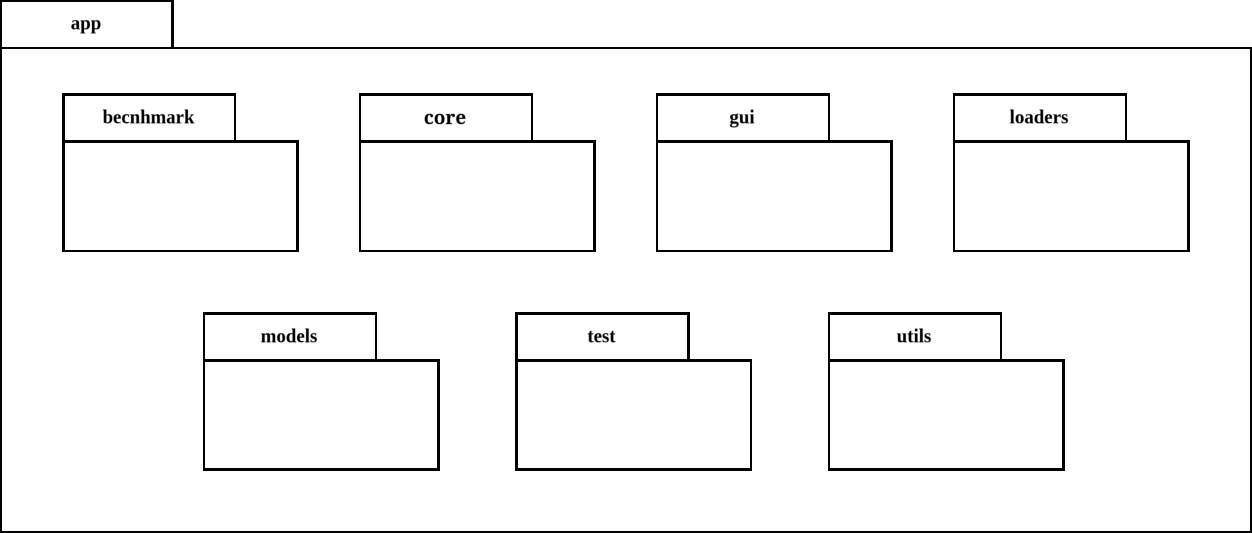
\includegraphics[width=0.95\textwidth]{sections/7/img/package_diagram.pdf}
    \caption{Diagrama de paquetes de la aplicación}
    \label{fig:54_package_diagram}
\end{figure}
